% Paper 1 -- main document. Introduction and Results 1 are drafted; later sections are stubs
% (their plan lives in schematic.tex). Every number in the text is a macro from numbers.tex,
% generated by ../1BQF_to_spectral_filter_corpus/13_paper_numbers.py.
\documentclass[11pt,a4paper]{article}
\usepackage[T1]{fontenc}\usepackage[utf8]{inputenc}\usepackage{lmodern}
\usepackage[margin=2.3cm]{geometry}
\usepackage{amsmath,amssymb}\usepackage{booktabs}\usepackage{graphicx}
\usepackage[labelfont=bf,font=small,skip=4pt]{caption}
\usepackage{subcaption}\usepackage{float}\usepackage{xcolor}
\usepackage[normalem]{ulem}% ulem.sty (CTAN 2019-11-18) copied next to main.tex: TeX Live on stbc lacks it
\usepackage{tikz}\usetikzlibrary{decorations.pathreplacing,calc}
% TikZ styles and helpers shared by figures/circuits.tex and figures/circuits_qsvt.tex
\tikzset{
  wire/.style={line width=0.55pt},
  gate/.style={draw,fill=white,minimum height=6.2mm,minimum width=7.5mm,inner sep=1.5pt,font=\small,line width=0.55pt},
  wgate/.style={gate,minimum width=13mm},
  ctrl/.style={circle,fill=black,inner sep=0pt,minimum size=1.9mm},
  octrl/.style={circle,draw,fill=white,inner sep=0pt,minimum size=1.9mm,line width=0.55pt},
  targ/.style={circle,draw,inner sep=0pt,minimum size=3.2mm,line width=0.55pt},
  meter/.style={draw,fill=white,minimum height=6.2mm,minimum width=7.5mm,line width=0.55pt},
  reg/.style={font=\small,anchor=east},
  blk/.style={font=\footnotesize,anchor=north,text=black!65},
  st/.style={font=\footnotesize,anchor=south,text=blue!45!black},
  brace/.style={decorate,decoration={brace,mirror,amplitude=2.2pt},line width=0.4pt,black!60},
  slash/.style={},
}
\newcommand{\slashwire}[3]{% x y label : the /n mark on a multi-qubit wire
  \draw[line width=0.7pt] (#1cm-1.3mm,#2cm-1.6mm) -- (#1cm+1.3mm,#2cm+1.6mm);
  \node[font=\scriptsize,anchor=south west,inner sep=0.4pt] at (#1cm+0.9mm,#2cm+0.9mm) {#3};}
\newcommand{\vsep}[3]{% x ybot ytop : a dashed block boundary
  \draw[dashed,black!45,line width=0.4pt] (#1cm,#2cm) -- (#1cm,#3cm);}


\usepackage{microtype}
\usepackage[colorlinks=true,linkcolor=blue!60!black,citecolor=green!45!black,urlcolor=blue!70!black]{hyperref}
\usepackage[numbers,sort&compress]{natbib}
\graphicspath{{figures/}}
% Generated by 1BQF_to_spectral_filter_corpus/13_paper_numbers.py -- do not edit by hand.
\newcommand{\NEvents}{10}
\newcommand{\NEventsTotal}{80}
\newcommand{\HitLossMean}{1.0}
\newcommand{\HitLossMin}{0.5}
\newcommand{\HitLossMax}{1.8}
\newcommand{\SigmaPMeas}{0.39}
\newcommand{\SigmaPPred}{0.40}
\newcommand{\CheckMaxDiff}{1e-7}
\newcommand{\EpsMrad}{1.70}
\newcommand{\EpsCos}{1.44\times10^{-6}}
\newcommand{\ResidualRms}{4.8}
\newcommand{\TrueOutside}{8.6\times10^{-5}}
\newcommand{\ClassFarTwoHundred}{0.12}
\newcommand{\OneBitFarTwoHundred}{0.12}
\newcommand{\QsvtEffTwoHundred}{0.984}
\newcommand{\QsvtEffMinTwoHundred}{0.969}
\newcommand{\QsvtFarTwoHundred}{0.56}
\newcommand{\ClassEffAtOneTwoHundred}{0.98}
\newcommand{\OneBitEffAtOneTwoHundred}{0.98}
\newcommand{\ClassFarFourHundred}{0.35}
\newcommand{\OneBitFarFourHundred}{0.35}
\newcommand{\QsvtEffFourHundred}{0.973}
\newcommand{\QsvtEffMinFourHundred}{0.938}
\newcommand{\QsvtFarFourHundred}{0.36}
\newcommand{\ClassEffAtOneFourHundred}{0.97}
\newcommand{\OneBitEffAtOneFourHundred}{0.49}
\newcommand{\ClassFarSevenHundred}{0.63}
\newcommand{\OneBitFarSevenHundred}{0.63}
\newcommand{\QsvtEffSevenHundred}{0.937}
\newcommand{\QsvtEffMinSevenHundred}{0.919}
\newcommand{\QsvtFarSevenHundred}{1.00}
\newcommand{\ClassEffAtOneSevenHundred}{0.49}
\newcommand{\OneBitEffAtOneSevenHundred}{0.49}
\newcommand{\ClassFarThousand}{0.77}
\newcommand{\OneBitFarThousand}{0.77}
\newcommand{\QsvtEffThousand}{0.917}
\newcommand{\QsvtEffMinThousand}{0.893}
\newcommand{\QsvtFarThousand}{1.00}
\newcommand{\ClassEffAtOneThousand}{0.24}
\newcommand{\OneBitEffAtOneThousand}{0.49}
\newcommand{\KeptPair}{0.38}
\newcommand{\KeptTriple}{0.53}
\newcommand{\KeptTrack}{0.59}
\newcommand{\KeptHubThree}{0.63}
\newcommand{\KeptHubFive}{0.77}
\newcommand{\AtlasPairs}{127{,}816}
\newcommand{\AtlasPairsKeptClass}{127{,}816}
\newcommand{\AtlasPairsKeptQsvt}{0}
\newcommand{\AtlasTriples}{5{,}074}
\newcommand{\AtlasTriplesKeptQsvt}{87}
\newcommand{\AtlasComplete}{35{,}952}
\newcommand{\AtlasCompleteKeptQsvt}{35{,}952}
\newcommand{\AtlasBroken}{1{,}057}
\newcommand{\AtlasBrokenLostQsvt}{1{,}057}
\newcommand{\AtlasContamLostQsvt}{2{,}222}
\newcommand{\IsolatedShare}{99.7}
\newcommand{\AtlasQsvtEff}{0.916}
\newcommand{\AtlasQsvtFar}{0.005}
\newcommand{\AtlasClassFar}{0.77}
\newcommand{\AtlasClassEff}{0.996}
\newcommand{\TrackInputWeightLow}{94.7}
\newcommand{\TrackSolutionWeightLow}{98.5}
\newcommand{\ContamNearTrue}{6}
\newcommand{\HubNearTrue}{88}
\newcommand{\TripleNearTrue}{0.7}
\newcommand{\QTrackLow}{0.995}
\newcommand{\QTrackHigh}{0.526}
\newcommand{\QIso}{0.007}
\newcommand{\QPairLow}{0.014}
\newcommand{\QPairHigh}{0.044}
\newcommand{\QTripleLow}{0.439}
\newcommand{\QTripleHigh}{0.198}
\newcommand{\QHubLow}{0.846}
\newcommand{\QHubHigh}{0.374}
\newcommand{\PairSuppression}{45}
\newcommand{\DomainLow}{0.24}
\newcommand{\DomainHigh}{7.76}
\newcommand{\DomainHalfWidth}{3.76}
\newcommand{\DomainLength}{7.52}
\newcommand{\ResolutionForty}{0.19}
\newcommand{\ResolutionSixty}{0.13}
\newcommand{\NIsolatedThousand}{39{,}077{,}686}
\newcommand{\TeethFourSeven}{0.935}
\newcommand{\TeethFourThousand}{0.928}
\newcommand{\TeethBrightThousand}{0.925}
\newcommand{\TeethDarkTwoHundred}{0.014}
\newcommand{\TeethDarkThousand}{0.000}
\newcommand{\TeethBestSeven}{0.960}
\newcommand{\TeethBestThousand}{0.951}
\newcommand{\TeethFourSixtySeven}{0.960}
\newcommand{\TeethFourSixtyThousand}{0.937}
\newcommand{\TeethNDesigns}{25}
\newcommand{\ClassCloseUpToT}{400}
\newcommand{\ClassDropT}{700}
\newcommand{\OneBitPlateau}{0.49}
\newcommand{\NSysFourHundred}{20}
\newcommand{\CxEvoFourHundred}{6.2\times10^{5}}
\newcommand{\CxHitFourHundred}{1.7\times10^{4}}
\newcommand{\WidthOneBitFourHundred}{22}
\newcommand{\POneBitFourHundred}{1.0\times10^{-3}}
\newcommand{\RoundsOneBitFourHundred}{24}
\newcommand{\TotalCallsOneBitFourHundred}{49}
\newcommand{\GatesEvoOneBitFourHundred}{3.0\times10^{7}}
\newcommand{\GatesHitOneBitFourHundred}{8.1\times10^{5}}
\newcommand{\WidthPhaseFourHundred}{24}
\newcommand{\PPhaseFourHundred}{4.1\times10^{-4}}
\newcommand{\RoundsPhaseFourHundred}{39}
\newcommand{\TotalCallsPhaseFourHundred}{6171}
\newcommand{\GatesEvoPhaseFourHundred}{3.8\times10^{9}}
\newcommand{\GatesHitPhaseFourHundred}{1.0\times10^{8}}
\newcommand{\WidthWalkFourHundred}{27}
\newcommand{\PWalkFourHundred}{1.1\times10^{-3}}
\newcommand{\RoundsWalkFourHundred}{24}
\newcommand{\TotalCallsWalkFourHundred}{1492}
\newcommand{\GatesEvoWalkFourHundred}{9.3\times10^{8}}
\newcommand{\GatesHitWalkFourHundred}{2.5\times10^{7}}
\newcommand{\WidthHhlFourHundred}{29}
\newcommand{\PHhlFourHundred}{1.3\times10^{-1}}
\newcommand{\RoundsHhlFourHundred}{2}
\newcommand{\TotalCallsHhlFourHundred}{1116}
\newcommand{\GatesEvoHhlFourHundred}{6.9\times10^{8}}
\newcommand{\GatesHitHhlFourHundred}{1.9\times10^{7}}
\newcommand{\NSysThousand}{22}
\newcommand{\CxEvoThousand}{2.0\times10^{6}}
\newcommand{\CxHitThousand}{3.6\times10^{4}}
\newcommand{\WidthOneBitThousand}{24}
\newcommand{\POneBitThousand}{8.6\times10^{-4}}
\newcommand{\RoundsOneBitThousand}{27}
\newcommand{\TotalCallsOneBitThousand}{54}
\newcommand{\GatesEvoOneBitThousand}{1.1\times10^{8}}
\newcommand{\GatesHitOneBitThousand}{1.9\times10^{6}}
\newcommand{\WidthPhaseThousand}{26}
\newcommand{\PPhaseThousand}{2.3\times10^{-4}}
\newcommand{\RoundsPhaseThousand}{52}
\newcommand{\TotalCallsPhaseThousand}{8315}
\newcommand{\GatesEvoPhaseThousand}{1.6\times10^{10}}
\newcommand{\GatesHitPhaseThousand}{3.0\times10^{8}}
\newcommand{\WidthWalkThousand}{29}
\newcommand{\PWalkThousand}{7.3\times10^{-4}}
\newcommand{\RoundsWalkThousand}{29}
\newcommand{\TotalCallsWalkThousand}{1838}
\newcommand{\GatesEvoWalkThousand}{3.6\times10^{9}}
\newcommand{\GatesHitWalkThousand}{6.6\times10^{7}}
\newcommand{\WidthHhlThousand}{31}
\newcommand{\PHhlThousand}{7.1\times10^{-2}}
\newcommand{\RoundsHhlThousand}{3}
\newcommand{\TotalCallsHhlThousand}{1499}
\newcommand{\GatesEvoHhlThousand}{3.0\times10^{9}}
\newcommand{\GatesHitHhlThousand}{5.4\times10^{7}}
\newcommand{\CallsOneBit}{2}
\newcommand{\CallsPhase}{160}
\newcommand{\CallsWalk}{63}
\newcommand{\CallsHhl}{510}
\newcommand{\PPhasePrefactor}{0.05}
\newcommand{\PPhaseExponent}{0.77}
\newcommand{\POneBitPrefactor}{0.05}
\newcommand{\POneBitExponent}{0.61}
\newcommand{\CxEvoPrefactor}{152}
\newcommand{\CxEvoExponent}{1.37}
\newcommand{\CxHitPrefactor}{103}
\newcommand{\CxHitExponent}{0.85}
\newcommand{\MeasuredTMax}{400}
\newcommand{\HitOracleAncillas}{45}
\newcommand{\ScanNEvents}{2}
\newcommand{\ScanClassTenUmTwoHundred}{0.25}
\newcommand{\ScanOneBitTenUmTwoHundred}{0.25}
\newcommand{\ScanQsvtTenUmTwoHundred}{0.94}
\newcommand{\ScanClassTenUmFourHundred}{0.49}
\newcommand{\ScanOneBitTenUmFourHundred}{0.49}
\newcommand{\ScanQsvtTenUmFourHundred}{0.90}
\newcommand{\ScanClassTenUmSevenHundred}{0.00}
\newcommand{\ScanOneBitTenUmSevenHundred}{0.00}
\newcommand{\ScanQsvtTenUmSevenHundred}{0.00}
\newcommand{\ScanClassTenUmThousand}{0.00}
\newcommand{\ScanOneBitTenUmThousand}{0.00}
\newcommand{\ScanQsvtTenUmThousand}{0.00}
\newcommand{\ScanClassFifteenUmTwoHundred}{0.33}
\newcommand{\ScanOneBitFifteenUmTwoHundred}{0.34}
\newcommand{\ScanQsvtFifteenUmTwoHundred}{0.57}
\newcommand{\ScanClassFifteenUmFourHundred}{0.00}
\newcommand{\ScanOneBitFifteenUmFourHundred}{0.12}
\newcommand{\ScanQsvtFifteenUmFourHundred}{0.47}
\newcommand{\ScanClassFifteenUmSevenHundred}{0.00}
\newcommand{\ScanOneBitFifteenUmSevenHundred}{0.00}
\newcommand{\ScanQsvtFifteenUmSevenHundred}{0.22}
\newcommand{\ScanClassFifteenUmThousand}{0.00}
\newcommand{\ScanOneBitFifteenUmThousand}{0.00}
\newcommand{\ScanQsvtFifteenUmThousand}{0.00}
\newcommand{\ScanClassThreeUmTwoHundred}{0.99}
\newcommand{\ScanOneBitThreeUmTwoHundred}{0.99}
\newcommand{\ScanQsvtThreeUmTwoHundred}{0.99}
\newcommand{\ScanClassThreeUmFourHundred}{0.98}
\newcommand{\ScanOneBitThreeUmFourHundred}{0.98}
\newcommand{\ScanQsvtThreeUmFourHundred}{0.98}
\newcommand{\ScanClassThreeUmSevenHundred}{0.98}
\newcommand{\ScanOneBitThreeUmSevenHundred}{0.74}
\newcommand{\ScanQsvtThreeUmSevenHundred}{0.98}
\newcommand{\ScanClassThreeUmThousand}{0.24}
\newcommand{\ScanOneBitThreeUmThousand}{0.24}
\newcommand{\ScanQsvtThreeUmThousand}{0.95}
\newcommand{\ScanClassFiveUmTwoHundred}{0.50}
\newcommand{\ScanOneBitFiveUmTwoHundred}{0.50}
\newcommand{\ScanQsvtFiveUmTwoHundred}{0.99}
\newcommand{\ScanClassFiveUmFourHundred}{0.98}
\newcommand{\ScanOneBitFiveUmFourHundred}{0.74}
\newcommand{\ScanQsvtFiveUmFourHundred}{0.98}
\newcommand{\ScanClassFiveUmSevenHundred}{0.24}
\newcommand{\ScanOneBitFiveUmSevenHundred}{0.49}
\newcommand{\ScanQsvtFiveUmSevenHundred}{0.94}
\newcommand{\ScanClassFiveUmThousand}{0.00}
\newcommand{\ScanOneBitFiveUmThousand}{0.25}
\newcommand{\ScanQsvtFiveUmThousand}{0.92}
\newcommand{\SegClassTau}{0.35}
\newcommand{\SegFarClassThousand}{0.13}
\newcommand{\SegFarOneBitThousand}{0.77}
\newcommand{\SegFarQsvtThousand}{0.39}
\newcommand{\CircuitCheckT}{3}
\newcommand{\CircuitCheckLo}{0.2}
\newcommand{\CircuitCheckHi}{7.8}
\newcommand{\CircuitCheckNSeg}{36}
\newcommand{\CircuitCheckErrEven}{2.2\times10^{-9}}
\newcommand{\CircuitCheckErrOdd}{1.6\times10^{-7}}
\newcommand{\PruneKeptFourHundred}{2{,}402}
\newcommand{\PruneQubitsFullFourHundred}{20}
\newcommand{\PruneQubitsFourHundred}{12}
\newcommand{\PruneQubitsThreeFourHundred}{11}
\newcommand{\PrunePGainFourHundred}{258}
\newcommand{\PruneRoundsGainFourHundred}{16}
\newcommand{\PruneOneBitEffFourHundred}{0.97}
\newcommand{\PruneOneBitT}{1.15}
\newcommand{\PruneKeptThousand}{17{,}092}
\newcommand{\PruneQubitsFullThousand}{22}
\newcommand{\PruneQubitsThousand}{15}
\newcommand{\PruneQubitsThreeThousand}{13}
\newcommand{\PrunePGainThousand}{224}
\newcommand{\PruneRoundsGainThousand}{15}
\newcommand{\PruneOneBitEffThousand}{0.49}
\newcommand{\PruneMinDegreeThousand}{20}

\newcommand{\eff}{\ensuremath{\varepsilon_{\rm seg}}}
\newcommand{\far}{\ensuremath{f_{\rm seg}}}
\makeatletter
\newlabel{fig:circuits}{{2}{}{}{}{}}
\newlabel{sec:fork:trotter}{{Methods}{}{}{}{}}
\makeatother

% Review mark-up (Oct 2026): JS = J. Schuetz (blue), MM = M. Merk (purple), GS = G. Scriven's replies (dark orange).
\newcommand{\js}[1]{{\color{blue} JS: #1 }}
\newcommand{\mm}[1]{{\color{purple} MM: #1 }}
\newcommand{\gs}[1]{{\color{orange!85!black} GS: #1 }}
\newcommand{\gss}[1]{{\color{teal} #1}}
% Redundancy pass (2026-10-27): \gsx = text proposed for removal (grey strike-through); gsxblock = a
% displayed equation proposed for removal (grey, no strike, since \sout cannot cross a display).
\newcommand{\gsx}[1]{{\color{gray}\sout{#1}}}
\newenvironment{gsxblock}{\color{gray}}{}
\newenvironment{gssblock}{\color{teal}}{}% a teal suggestion that contains displayed equations
\newcommand{\R}{\mathbb{R}}

\title{From one bit to any polynomial:\\ quantum spectral filters for track finding in the LHCb vertex detector}
\author{G.\,W.\,Scriven, X.\,Chiotopoulos, D.\,Nicotra, J.\,Sch\"utz, J.\,de\,Vries, M.\,Merk\\
\small (author list and affiliations to be agreed)}
\date{Draft, \today}

\begin{document}
\maketitle

\begin{abstract}
\noindent\textit{Draft, to be finalised with the results sections.}
The one-bit quantum filter reconstructs particle-track segments by applying one cosine of a
segment Hamiltonian, which removes the isolated false segments at a small fraction of the cost
of quantum phase estimation. On simulated events with detector noise it keeps a high
efficiency, but a false rate of $\OneBitFarFourHundred$ at 400 tracks and $\OneBitFarThousand$
at 1000. We show that the filter is the degree-one member of the polynomial transforms
provided by the quantum singular value transformation, and that a degree-40 polynomial on the
same Hamiltonian keeps $\QsvtEffThousand$ of true segments at a false rate below $1\%$ at 1000
tracks. We identify which configurations each filter keeps from their eigenvalues alone, and
give the cost of the polynomial in calls, gates and qubits.
\end{abstract}

\section{Introduction}

\mm{@George, before removing suggested text, please first address suggestions in the comment panel otherwise we may not agree and keep oscillating.}\\

\mm{@George: please also focus on academic tone, avoiding colloquial language and make sure that the meaning of every word is precisely defined.}\\

\mm{I previously added some explanatory text and connection to previous papers: whenever we use things like "isolated segments" they are not yet defined and not understood unless defined. Hence, I do think we need the schematic illustration added below....} \gs{Implemented. This Introduction now defines each term before its first use, links the work to refs.~\cite{nicotra2023,trackhhl} and ends with the motivation for a response with more than one zero. The schematic is figure~\ref{Fig:ToyEvent}.}
\mm{In case we are not aiming the article for JINST (particle physics instrumentation) I still think we need to explain more introductory. A bunch is not defined, a hit is not defined, a track is not defined and I has defined those before. We cannot leave that out.} \gs{Accepted. I suggest the definitions of bunch crossing, hit and track at the start of the Introduction, before their first use. I used your wording from the previous round where possible.}

\gss{At the LHC, protons collide in bunches, and each bunch crossing produces many charged particles. Each particle crosses the layers of the detector and leaves a set of spatial measurements, called hits. A track is the set of hits left by one particle. Track finding is the task of grouping the hits of a bunch crossing into tracks.} At the High-Luminosity LHC a single bunch crossing will leave thousands of charged-particle hits
in the LHCb vertex detector. The first step \mm{(step of what? --> undefined)} \gs{Accepted. I suggest stating that it is the first step of event reconstruction, before the track fit.} of reconstruction is to connect the hits that belong to
the same particle. This step is track finding. \gss{Track finding is the first step of event reconstruction: it groups the hits into tracks before the track parameters are fitted.} It is a pattern-recognition problem, and its complexity
grows quadratically with the number of particles. Between two detector planes with $T$ \mm{strange to call the number of hits $T$ - need to reformulate} hits each there are
$T^2$ pairs of hits, but only $T$ pairs belong to the same particle. We call a pair of hits on
adjacent planes a candidate segment, and a candidate that is correctly assigned to a particle track a true segment
(figure~\ref{Fig:ToyEvent}a). The search for correct track segments is then a search for $T$ true segments in a
background of $T^2-T$ false candidates, and the background grows quadratically with the number of
particles.
\mm{The definition of $T$ is a bit problematic since you assume that all hits are part of a correct segment.}
\gss{Consider an event with $T$ particle tracks. If each track leaves one hit on each detector plane, two adjacent planes carry $T$ hits each. They form $T^2$ pairs of hits, of which only $T$ belong to the same particle. In a real detector some hits are lost, so this count holds only approximately, but the quadratic growth of the false candidates is unchanged.}

\begin{figure}[H]\centering
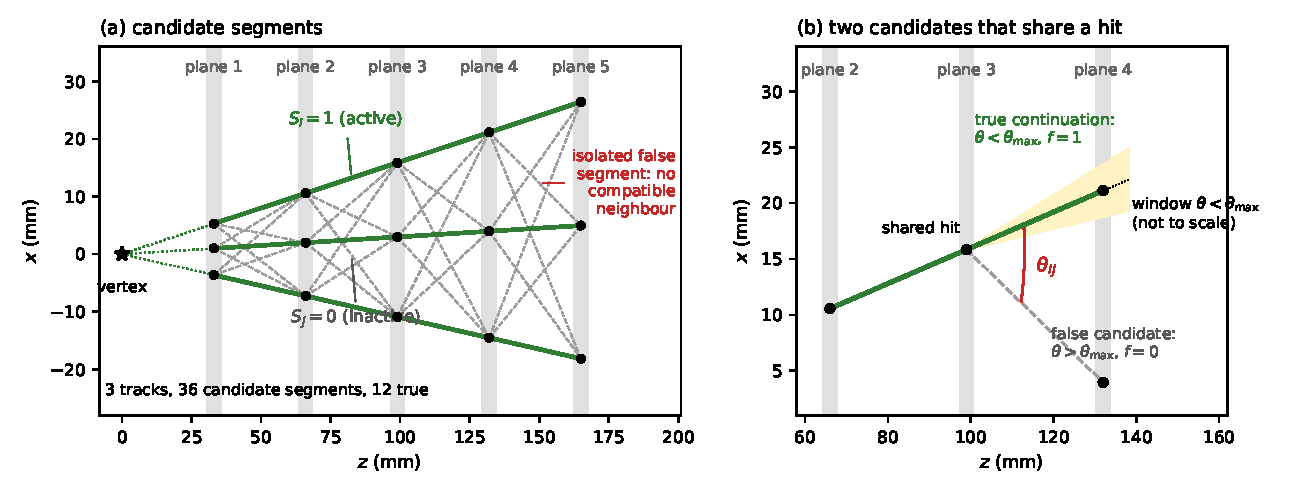
\includegraphics[width=0.95\textwidth]{fig0_toy_scheme.pdf}
\caption{\textbf{Candidate segments in a small event.} (a)~Three straight tracks from one vertex
cross five planes. Each pair of hits on adjacent planes is a candidate segment. The segments of the
true tracks are active ($S_i=1$, green). All other candidates are inactive ($S_j=0$, grey). In this
event no false candidate has a compatible neighbour, so each false candidate is an isolated false
segment. (b)~Two candidates that share one hit. The angle $\theta_{ij}$ between them is the kink.
The two segments are compatible ($f=1$) when the kink is smaller than $\theta_{\max}$. The window is
drawn much wider than the real $\theta_{\max}=\EpsMrad$\,mrad.}
\label{Fig:ToyEvent}
\end{figure}

Track finding is one of the few reconstruction tasks that can be written as linear algebra.\mm{this statement "hangs" a bit here and should go elsewhere.} Following the method of Denby
and Peterson we give each candidate segment a binary variable $S_i$ and write track finding as the
minimisation of a Hamiltonian  defined quadratically in these variables~\cite{denby1988,peterson1989}. The energy
rewards two subsequent segments that share a hit and only make a small kink
(figure~\ref{Fig:ToyEvent}b); we call two such segments compatible. When the variables are relaxed
to real numbers \mm{this remark is strange here, turn the sentences around: "In earlier work we showed that relaxing the binary variables $S_i$ to real numbers...."}, the minimum of the energy is the solution of a linear system, and the solution
gives every segment a score. \gss{In earlier work we showed that relaxing the binary variables $S_i$ to real numbers turns the minimisation into a linear system, so that track finding becomes a problem of linear algebra~\cite{nicotra2023}. The solution of this system gives every segment a score.} In earlier work we solved this system with the
Harrow--Hassidim--Lloyd (HHL) algorithm~\cite{hhl2009,nicotra2023}. The matrix fulfills two essential
conditions that are HHL requires to be successful: its sparsity increases with the problem size, and its condition number
stays bounded. Under these conditions HHL promises a run time that grows with the logarithm of the
number of segments. The resulting circuit size, however, was beyond the possibilies of near-term hardware. High-precision phase
estimation resulted in very deep circuits, and the final state tomography at readout required too many samples.

Track finding does not need the precise values of the solution. It needs only to know which
segments are active. This observation led to the development of the one-bit quantum
filter~\cite{trackhhl_epj,trackhhl}. 
The filter restricts phase estimation to a single bit; a
single-ancilla circuit that applies one cosine of the Hamiltonian \mm{makes no sense: this cosine is not present in the Hamiltonian! I suggest: "The filter restricts phase estimation to a single bit and is tuned to filter out eigenstates that correspond to isolated (false) segments} \gss{The filter restricts phase estimation to a single bit and is tuned to filter out the eigenstates that correspond to isolated false segments. Its single-ancilla circuit has a response that is a cosine of the eigenvalue, with the zero of the cosine placed on the eigenvalue shared by every isolated false segment: a false candidate with no compatible neighbour (figure~\ref{Fig:ToyEvent}a).}, with the zero of the cosine
placed on one eigenvalue. This eigenvalue is shared by every isolated false segment: a false
candidate with no compatible neighbour (figure~\ref{Fig:ToyEvent}a). The filter requires only two calls to
the time evolution, where phase estimation needs hundreds. \mm{can you substantiate this comment? I am surprised this is the case for say 3 bits.} \gss{The filter requires only two calls to the time evolution per shot. Phase estimation with the eight bits of our earlier work requires $\CallsHhl$, because each bit doubles the number of controlled calls, and fewer bits do not resolve the eigenvalues that HHL must invert.} It removes most of the false candidates
before readout, and it was validated for small simulations of trackfinding against the noise models of trapped-ion and superconducting
processors~\cite{trackhhl}. \mm{not only noise models! also at actual hardware!} \gss{It removes most of the false candidates before readout, and it was validated for small simulations of track finding both against the noise models of trapped-ion and superconducting processors and on the processors themselves~\cite{trackhhl}.}

The one-bit filter makes a simple spectral selection: it removes one eigenvalue. At low densities of tracks in the detectors
this may be sufficient, because almost every false candidate is an isolated segment. At realistic conditions of the
High-Luminosity LHC it is not sufficient. False candidates then also form pairs, triples and hubs of
compatible segments, and each of these groups has its own eigenvalues. \mm{pairs, triples and hubs are not defined. At this point we should keep the text a bit more general and avoid naming specific topologies.} \gss{False candidates then also form groups of compatible segments. Each group is a small graph of segments, and each kind of group has its own eigenvalues. One zero cannot remove them all.} One zero cannot remove them
all. On our simulated events the isolated false segments make up $\IsolatedShare\%$ of all false
candidates at 1000 tracks, and this share is a property of the geometry: a false candidate couples
to another only when a third hit lies inside a narrow angular window. \js{Is this true in general? Or only for a toy problem?} \gs{The number is for my events; the sentence now gives the geometric argument. The share increases with $T$ at a fixed window.} 
\mm{I agree with JS that it makes no sense to quote numbers here. The idea is generic and the numbers are completely defined by the number of particles, their distribution  and the size of the acceptance window. In other words, at this point fully tuneable. Don't mention them.} \gss{On simulated events the isolated false segments are the large majority of all false candidates, and this is a property of the geometry: a false candidate couples to another only when a third hit lies inside a narrow angular window.}
The
remaining fraction, however, decides the false rate. Read where it keeps $99\%$ of true segments,
the one-bit filter has the same false rate as the classical solver on events with detector noise:
$\OneBitFarFourHundred$ at 400 tracks and $\OneBitFarThousand$ at 1000 (table~\ref{tab:headline}).
Here the false rate is the fraction of the kept segments that are false, and the classical solver
is the direct solution of the linear system, read at a threshold on the score~\cite{nicotra2023,trackhhl}.
\js{Where are these numbers from? Cite or explain.} \gs{Now referenced to table~\ref{tab:headline}; all numbers come from the events of section~\ref{sec:r1}.}
\mm{At this point in the paper there is no need for these numbers. They are misleading and fully tuneable. Just keep the text generic, which is enough for the motivation. For example we can just say: The number of incorrect segments were observed to rise for high particle multiplicities." This is exactly the plot in the previous paper. (And will get much worse for even higher multiplicities that are needed.)} \gss{The remaining fraction, however, decides the false rate. In our earlier work the number of incorrect segments kept by the filter was observed to rise with the particle multiplicity~\cite{trackhhl}, and it rises further at the multiplicities of the High-Luminosity LHC.}

This motivates a spectral filter with more than one zero. The quantum singular value transformation
(QSVT)~\cite{gslw2019,martyn2021} provides a method to implement this. The QSVT applies to a Hamiltonian any polynomial
bounded by 1 on $[-1,1]$, at a cost linear in the degree of the polynomial. \js{A difficult statement for a mathematician ;-) Also, how is it connected to the rest?} \gs{Rewritten: the one-bit response has one zero in the spectrum; a QSVT response of degree $d$ has up to $d$.  } \js{there is no such thing as a bounded polynomial, save the constant} \gs{Corrected to `bounded by 1 on $[-1,1]$'.} 
\mm{I am also confused: the QSVT does not apply to the "Hamiltonian"?} \gss{The QSVT takes a block encoding of the Hamiltonian and applies a polynomial of our choice to its eigenvalues. Any polynomial bounded by 1 on $[-1,1]$ is allowed, at a cost linear in its degree. The one-bit filter is the degree-one member of this family.} The response of the
filter can be designed as it can pass the eigenvalues of true track segments and reject several classes of
false groups at the same time, in addition to  isolated segments. The one-bit filter is the degree-one member of this
family. It is the starting point of this paper, and the QSVT is the framework in which we build the
general filter.

In this paper we use this generalisation. We show that the true tracks of the detector occupy a small set
of known eigenvalues. We design a polynomial that passes these eigenvalues and rejects the rest. On
simulated events with detector noise it keeps a comparable efficiency ($\QsvtEffThousand$ at 1000
tracks) and reduces the false rate to below $1\%$. \mm{Also don't put numbers here - not needed and does not really help.} \gss{On simulated events with detector noise it keeps a comparable efficiency and reduces the false rate well below that of the one-bit filter.} We identify from the eigenvalues alone which
configurations each filter keeps, and why. The price is a deeper circuit and, for the block encoding
that makes it efficient, more qubits. Section~\ref{sec:r4} quantifies both costs: the number of logical qubits and the number of two-qubit gates per solved event.


\gs{The teal roadmap below replaces this sentence and the placeholder; marked for removal.} \gsx{Section~\mbox{\ref{sec:r1}} builds the problem from a noisy event: the detector model, the acceptance
window, the Hamiltonian, the one-bit filter, and what each solver keeps.}
\gsx{\textit{[Sections on the spectrum, the polynomial, results against multiplicity and cost follow;
see schematic.tex.]}}

\gss{Section~\ref{sec:methods} gives the detector simulation, the acceptance window, the Hamiltonian, the circuits of the one-bit filter and of the polynomial filter, and the cost model. Section~\ref{sec:r1} then builds the problem from a noisy event, section~\ref{sec:r2} designs the polynomial from the spectrum, section~\ref{sec:r3} gives the results against track multiplicity, and section~\ref{sec:r4} the computational cost.}

\section{Methods}\label{sec:methods}

\subsection{Detector simulation and the set of events}\label{sec:m:events}
Five planes at $z=33,66,99,132$ and $165$\,mm. $T$ tracks per event from the origin, with
directions uniform in a cone of half-opening $0.2$\,rad. One hit per track per plane. Three effects
in this order: a multiple-scattering kink with Gaussian projections of width $\sigma_{\rm scatt}=0.15$\,mrad
at each plane; Gaussian smearing of each hit with $\sigma_{\rm res}=5\,\mu$m in $x$ and $y$; removal of
each hit with probability $0.01$. $\NEvents$ events for each of $T=10,20,50,100,200,400,700,1000$,
$\NEventsTotal$ events in all. On the set the measured hit residuals are $\ResidualRms\,\mu$m and the
hit loss is $\HitLossMean\%$ on average, between $\HitLossMin\%$ and $\HitLossMax\%$ per event.
Six checks run on every event and the build stops on a failure: the classical solution against an
iterative solve of the full sparse system; the one-bit amplitudes against the sparse matrix
exponential; the polynomial against the Chebyshev recursion on the full matrix; every entry of $C$
against the stored segment directions; the closed-form values $4/11$, $5/11$ and $1/4$ on isolated
tracks and segments; and the measured noise against its prediction. The largest difference in the
first three checks is $\CheckMaxDiff$.

\subsection{The acceptance window}\label{sec:m:window}
\gss{A candidate segment is a pair of hits on adjacent planes (figure~\ref{Fig:ToyEvent}a). Each candidate carries a variable $S_i\in\{0,1\}$, $i=1,\dots,N$, with $S_i=1$ for an active segment. The index $i$ runs over all candidates, not over tracks. A segment joins plane $k$ to plane $k+1$, so the plane index is implicit in $i$, and two segments share a hit only when one ends on the plane where the other starts. With no hit loss there are $N=4T^2$ candidates; with hit loss $N\approx4T^2$. A true segment is a candidate whose two hits belong to the same particle; every other candidate is false. A true continuation is a pair of segments of the same track on three consecutive planes $k$, $k+1$ and $k+2$. Without noise it is a straight line; with noise the second segment turns by a small angle, the kink $\theta_{ij}$ (figure~\ref{Fig:ToyEvent}b).}

Three hits of one track at $x_1,x_2,x_3$ on consecutive planes give the kink projection
$(x_1-2x_2+x_3)/\Delta z$. With independent position errors of width $\sigma_{\rm res}$ and a
scattering kink of width $\sigma_{\rm scatt}$ at the middle plane, the projection has variance
$\sigma_p^2=\sigma_{\rm scatt}^2+6\sigma_{\rm res}^2/\Delta z^2$. The $x$ and $y$ projections are
independent, so the kink magnitude follows a Rayleigh law with
$P(\theta>\theta_{\max})=\exp[-\theta_{\max}^2/(2\sigma_p^2)]$. We set $\theta_{\max}=3\sqrt2\sigma_p$,
which loses $e^{-9}$ of true continuations, and $\varepsilon=1-\cos\theta_{\max}$. \gss{At the detector of section~\ref{sec:m:events} this gives $\theta_{\max}=\EpsMrad$\,mrad and $\varepsilon=\EpsCos$. Two segments $i$ and $j$ that share a hit are compatible when their kink is inside the window,
\begin{equation}
f(\theta_{ij},\varepsilon)=\begin{cases}1,&\cos\theta_{ij}\ge1-\varepsilon,\\0,&\text{otherwise},\end{cases}
\end{equation}
and a false candidate with no compatible neighbour is an isolated false segment (figure~\ref{Fig:ToyEvent}a).}
\gs{Kept in section~\mbox{\ref{sec:r1}} with figure~\mbox{\ref{fig:hits}}b; marked for removal here.} \gsx{On the set the
measured width of true continuations is $\SigmaPMeas$\,mrad against $\SigmaPPred$\,mrad predicted,
and $\TrueOutside$ of true continuations fall outside the window.}

\subsection{The Hamiltonian and the classical solver}\label{sec:m:hamiltonian}
\gs{Now defined in section~\mbox{\ref{sec:m:window}}; marked for removal here.} \gsx{A candidate segment is a pair of hits on adjacent planes; with no hit loss there are $N=4T^2$.}
\gss{Track finding is the search for the ground state of the Hamiltonian of refs.~\cite{nicotra2023,trackhhl} over the vector $S\in\{0,1\}^N$,
\begin{equation}
\mathcal{H}(S)=\mathcal{H}_{\rm ang}(S,\varepsilon)+\alpha\,\mathcal{H}_{\rm spec}(S)+\beta\,\mathcal{H}_{\rm gap}(S),
\end{equation}
\begin{equation}
\mathcal{H}_{\rm ang}(S,\varepsilon)=-\frac12\sum_{i,j}f(\theta_{ij},\varepsilon)\,S_iS_j,\qquad
\mathcal{H}_{\rm spec}(S)=\frac12\sum_i S_i^2,\qquad
\mathcal{H}_{\rm gap}(S)=\frac12\sum_i\big(1-S_i\big)^2 .
\end{equation}
The angular term rewards compatible continuations (figure~\ref{Fig:ToyEvent}b), and the two regularisation terms keep the problem well posed. Ref.~\cite{trackhhl} writes $\mathcal{H}_{\rm spec}$ and $\mathcal{H}_{\rm gap}$ without the factor $\frac12$; the factor, which its reference implementation carries, is what gives the diagonal $\alpha+\beta$ and $\mathbf{b}=\beta\,\mathbf{1}$ stated there. The function $f$ acts on the measured angles, which are data fixed before the solve, so the energy is quadratic in $S$. Relaxing $S$ to a real vector $\mathbf{x}\in\R^N$, the minimum is where the gradient, which is linear in $\mathbf{x}$, vanishes:
\begin{equation}
\label{eq:Axb:methods}
\nabla_{\mathbf{x}}\mathcal{H}=A\mathbf{x}-\mathbf{b}=0,
\end{equation}
where $\mathbf{1}$ is the vector of $N$ ones. We take $\alpha=3$ and $\beta=1$ (ref.~\cite{trackhhl} used $\alpha=2$).}
The
compatibility matrix $C$ has $C_{ij}=1$ when segments $i$ and $j$ share a hit and their kink is
below $\theta_{\max}$, and $0$ otherwise. $A=\lambda_cI-C$ with $\lambda_c=\alpha+\beta=4$ and
$\mathbf{b}=\beta\mathbf{1}$ with $\beta=1$. The connected groups of compatible segments are found
once per event; every solver works on the same groups. The classical solution is
$\mathbf{x}=A^{-1}\mathbf{b}$, computed on each group from its eigenvalues and eigenvectors. An
isolated segment solves to $\beta/\lambda_c$; a chain of $m$ segments solves to
$\sum_k\langle\mathbf{v}_k,\mathbf{b}\rangle\mathbf{v}_k/\lambda_k$ with
$\lambda_k=\lambda_c-2\cos(k\pi/(m+1))$ and $v_{k,j}\propto\sin(kj\pi/(m+1))$.

\subsection{The one-bit filter: circuit and state}\label{sec:m:onebit}
The segment register $S$ has $n=\lceil\log_2N\rceil$ qubits. $A$ is padded to $2^n$ rows with
diagonal entries $\lambda_c$ and $\mathbf{b}$ with ones, so each padding state is an isolated
segment and the zero of the filter removes it. The flag $A$ and the phase bit $T$ start in $|0\rangle$. \gss{The segment register starts in the uniform state $|u\rangle=\frac{1}{\sqrt N}\sum_{i=1}^{N}|i\rangle$ over the candidate segments, with amplitude vector $\mathbf{u}$, $u_i=1/\sqrt N$.}
The states of figure~\ref{fig:filters}a are
\begin{align}
|\Psi_1\rangle&=|0\rangle_A|0\rangle_T|u\rangle,\\
|\Psi_2\rangle&=|0\rangle_A\otimes\Big[|0\rangle_T\otimes\tfrac12(I+e^{-iAt})|u\rangle+|1\rangle_T\otimes\tfrac12(I-e^{-iAt})|u\rangle\Big],\\
|\Psi_3\rangle&=|1\rangle_A|0\rangle_T\otimes\tfrac12(I+e^{-iAt})|u\rangle+|0\rangle_A|1\rangle_T\otimes\tfrac12(I-e^{-iAt})|u\rangle,\\
|\Psi_4\rangle&=|1\rangle_A\otimes\Big[|0\rangle_T\otimes\cos^2\!\big(\tfrac{At}{2}\big)|u\rangle-\tfrac{i}{2}|1\rangle_T\otimes\sin(At)|u\rangle\Big]\nonumber\\
&\qquad-|0\rangle_A\otimes\Big[|0\rangle_T\otimes\sin^2\!\big(\tfrac{At}{2}\big)|u\rangle+\tfrac{i}{2}|1\rangle_T\otimes\sin(At)|u\rangle\Big],
\end{align}
using $\tfrac12(I+e^{-iAt})=e^{-iAt/2}\cos(At/2)$ and $\tfrac12(I-e^{-iAt})=-ie^{-iAt/2}\sin(At/2)$.
$|\Psi_2\rangle$ follows from the Hadamard, the controlled $e^{-iAt}$ and the Hadamard on $T$;
$|\Psi_3\rangle$ from the flag, a NOT on $A$ controlled on $T=0$; $|\Psi_4\rangle$ from the same
three gates with $e^{+iAt}$. Post-selection on $A=1$ succeeds with probability
$\langle u|\cos^2(At/2)|u\rangle$ and reads segment $i$ with probability
$p_i=[\cos^2(At/2)\mathbf{u}]_i^2+[\tfrac12\sin(At)\mathbf{u}]_i^2$. With $t=\pi/\lambda_c$ the zero
of $\cos(\lambda t/2)$ lies at $\lambda=\lambda_c$. The amplitudes in this paper are $\sqrt{p_i}$,
computed exactly on each group. \gss{On an eigencomponent of $A$ with eigenvalue $\lambda$ the amplitude is multiplied by $\cos(\lambda t/2)$, and the probability weight by its square: the sine term carries the same factor, since $\tfrac12\sin(\lambda t)=\cos(\lambda t/2)\sin(\lambda t/2)$. Every isolated segment has the eigenvalue $\lambda_c$ (section~\ref{sec:r1}), so the zero removes it exactly.}

% Moved here from section sec:r1 (redundancy pass, 2026-10-27); caption unchanged.
\begin{figure}[H]
\centering
\resizebox{0.95\textwidth}{!}{% Figure 2 of paper 1 (16 Sep 2026): the one-bit filter, and the QSVT with the dilation encoding.
% Built from circuits.tex panel (b) and circuits_qsvt.tex panel (a); requires circuit_styles.tex.
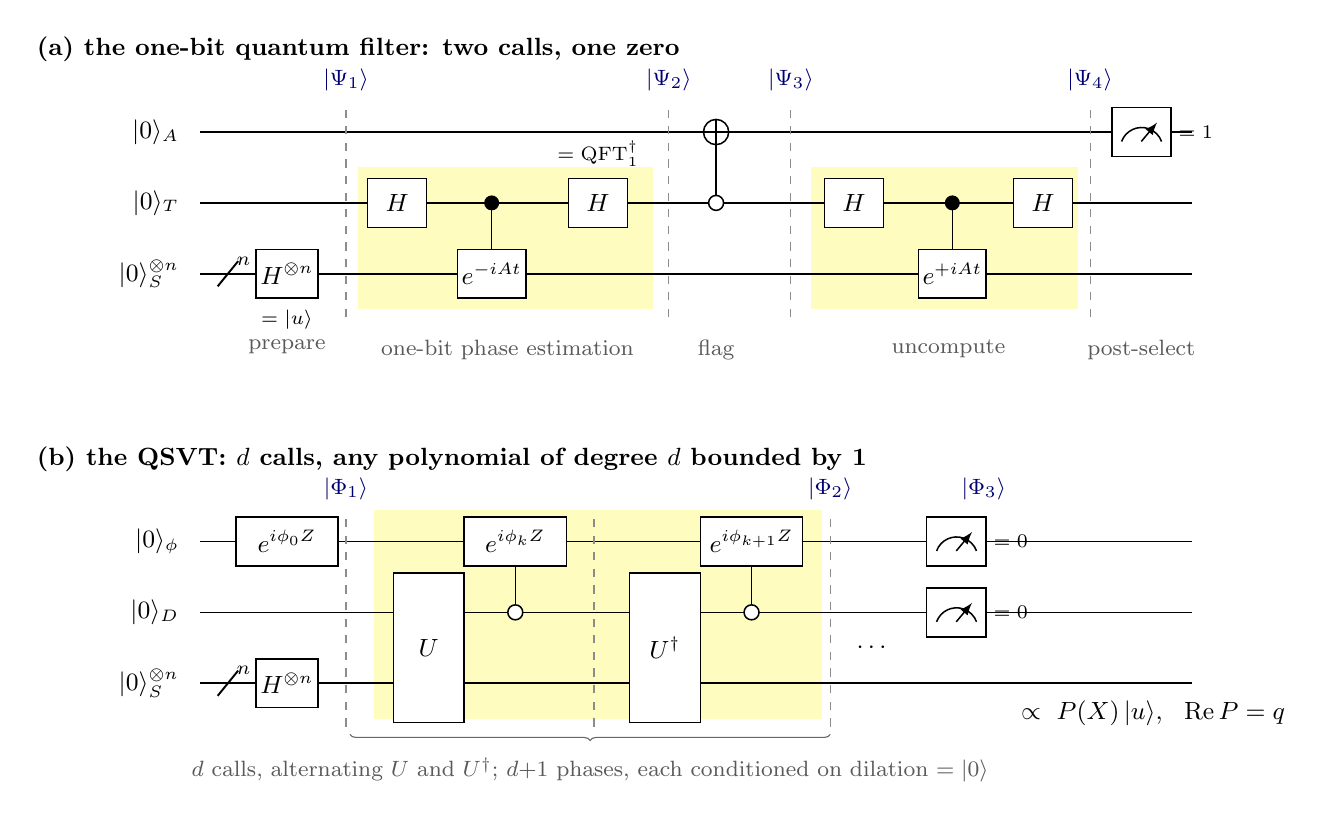
\begin{tikzpicture}[x=1cm,y=1cm]
\begin{scope}[shift={(0,0)}]
\fill[yellow!25] (2.0,-1.35) rectangle (5.75,0.45); \fill[yellow!25] (7.75,-1.35) rectangle (11.15,0.45);
\node[anchor=west,font=\small\bfseries] at (-2.2,1.95) {(a) the one-bit quantum filter: two calls, one zero};
\node[reg] at (-0.15,0.9)  {$|0\rangle_{A}$};
\node[reg] at (-0.15,0)    {$|0\rangle_{T}$};
\node[reg] at (-0.15,-0.9) {$|0\rangle^{\otimes n}_{S}$};
\draw[wire] (0,0.9) -- (12.6,0.9); \draw[wire] (0,0) -- (12.6,0); \draw[wire] (0,-0.9) -- (12.6,-0.9);
\slashwire{0.35}{-0.9}{$n$}
\node[gate] at (1.1,-0.9) {$H^{\otimes n}$};
\node[font=\scriptsize,anchor=north] at (1.1,-1.24) {$=|u\rangle$};
\vsep{1.85}{-1.45}{1.25}
\node[gate] at (2.5,0) {$H$};
\node[ctrl] at (3.7,0) {}; \draw[wire] (3.7,0) -- (3.7,-0.9); \node[gate] at (3.7,-0.9) {$e^{-iAt}$};
\node[gate] at (5.05,0) {$H$};
\node[font=\scriptsize,anchor=south] at (5.05,0.34) {$=\mathrm{QFT}_1^{\dagger}$};
\vsep{5.95}{-1.45}{1.25}
\node[octrl] at (6.55,0) {}; \draw[wire] (6.55,0.09) -- (6.55,0.9); \node[targ] at (6.55,0.9) {}; \draw[wire] (6.55,0.74) -- (6.55,1.06);
\vsep{7.5}{-1.45}{1.25}
\node[gate] at (8.3,0) {$H$};
\node[ctrl] at (9.55,0) {}; \draw[wire] (9.55,0) -- (9.55,-0.9); \node[gate] at (9.55,-0.9) {$e^{+iAt}$};
\node[gate] at (10.7,0) {$H$};
\vsep{11.3}{-1.45}{1.25}
\node[meter] at (11.95,0.9) {}; \draw[wire] (11.7,0.78) arc (160:20:0.27); \draw[wire,-latex] (11.95,0.78) -- (12.15,1.02);
\node[font=\scriptsize,anchor=west] at (12.3,0.9) {$=1$};
\node[blk] at (1.1,-1.62) {prepare};
\node[blk] at (3.9,-1.62) {one-bit phase estimation};
\node[blk] at (6.55,-1.62) {flag};
\node[blk] at (9.5,-1.62) {uncompute};
\node[blk] at (11.95,-1.62) {post-select};
\node[st] at (1.85,1.3) {$|\Psi_1\rangle$}; \node[st] at (5.95,1.3) {$|\Psi_2\rangle$};
\node[st] at (7.5,1.3) {$|\Psi_3\rangle$}; \node[st] at (11.3,1.3) {$|\Psi_4\rangle$};
\end{scope}
\begin{scope}[shift={(0,-5.2)}]
\fill[yellow!25] (2.2,-1.35) rectangle (7.9,1.3);
\node[anchor=west,font=\small\bfseries] at (-2.2,1.95) {(b) the QSVT: $d$ calls, any polynomial of degree $d$ bounded by 1};
\node[reg] at (-0.15,0.9)  {$|0\rangle_{\phi}$};
\node[reg] at (-0.15,0)    {$|0\rangle_{D}$};
\node[reg] at (-0.15,-0.9) {$|0\rangle^{\otimes n}_{S}$};
\draw[wire] (0,0.9) -- (12.6,0.9); \draw[wire] (0,0) -- (12.6,0); \draw[wire] (0,-0.9) -- (12.6,-0.9);
\slashwire{0.35}{-0.9}{$n$}
\node[gate] at (1.1,-0.9) {$H^{\otimes n}$};
\node[gate,minimum width=13mm] at (1.1,0.9) {$e^{i\phi_0 Z}$};
\vsep{1.85}{-1.45}{1.25}
% one repetition: U on (D,S), then the projector-controlled phase on the signal qubit
\node[gate,minimum height=19mm,minimum width=9mm] at (2.9,-0.45) {$U$};
\node[octrl] at (4.0,0) {}; \draw[wire] (4.0,0.09) -- (4.0,0.62);
\node[gate,minimum width=13mm] at (4.0,0.9) {$e^{i\phi_k Z}$};
\vsep{5.0}{-1.45}{1.25}
\node[gate,minimum height=19mm,minimum width=9mm] at (5.9,-0.45) {$U^{\dagger}$};
\node[octrl] at (7.0,0) {}; \draw[wire] (7.0,0.09) -- (7.0,0.62);
\node[gate,minimum width=13mm] at (7.0,0.9) {$e^{i\phi_{k+1} Z}$};
\vsep{8.0}{-1.45}{1.25}
\node[font=\small] at (8.55,-0.45) {$\cdots$};
\draw[brace] (1.9,-1.55) -- (8.0,-1.55); \node[blk] at (4.95,-1.72) {$d$ calls, alternating $U$ and $U^{\dagger}$; $d{+}1$ phases, each conditioned on dilation $=|0\rangle$};
\node[meter] at (9.6,0.9) {}; \draw[wire] (9.35,0.78) arc (160:20:0.27); \draw[wire,-latex] (9.6,0.78) -- (9.8,1.02);
\node[font=\scriptsize,anchor=west] at (9.95,0.9) {$=0$};
\node[meter] at (9.6,0) {}; \draw[wire] (9.35,-0.12) arc (160:20:0.27); \draw[wire,-latex] (9.6,-0.12) -- (9.8,0.12);
\node[font=\scriptsize,anchor=west] at (9.95,0) {$=0$};
\node[font=\small,anchor=north west] at (10.3,-1.0) {$\propto\ P(X)\,|u\rangle,\ \ \mathrm{Re}\,P=q$};
\node[st] at (1.85,1.3) {$|\Phi_1\rangle$}; \node[st] at (8.0,1.3) {$|\Phi_2\rangle$}; \node[st] at (9.95,1.3) {$|\Phi_3\rangle$};
\end{scope}
\end{tikzpicture}
}\\[6pt]
\begin{minipage}{0.70\textwidth}\centering
{\small\bfseries (c)}\\
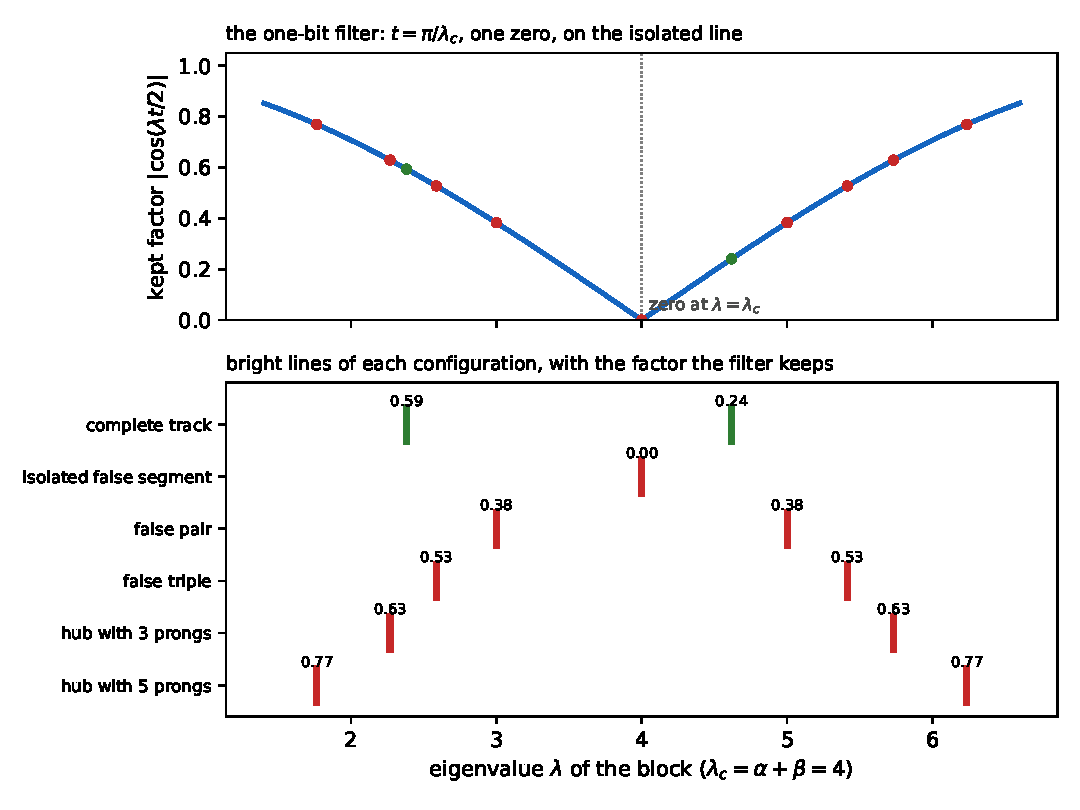
\includegraphics[width=\textwidth]{fig2_onebit_response.pdf}
\end{minipage}
\caption{\textbf{One zero, and any polynomial.} (a)~The one-bit filter: one bit of phase
estimation with two calls to the controlled evolution (highlighted) applies $\cos(\lambda t/2)$,
with a single zero at $\lambda=\lambda_c$. (b)~The quantum singular value transformation: $d$ calls to a
block encoding $U$ of $A$ (highlighted), with a phase rotation between calls, apply any
polynomial of degree $d$ bounded by 1 on $[-1,1]$. Here $U$ is the dilation
$U=\bigl(\begin{smallmatrix}X&\sqrt{I-X^2}\\ \sqrt{I-X^2}&-X\end{smallmatrix}\bigr)$ of
$X=(A-c_0I)/c_1$; a block encoding priced by detector hits is introduced later. (c)~The factor
the one-bit filter keeps on the eigenvalues of each segment class.}
\label{fig:filters}
\end{figure}

\subsection{Polynomial design and phase factors}\label{sec:m:polynomial}
The target is $g(\lambda)$ of section~\ref{sec:r2}: four Gaussian passes of half-width $h=0.18$ on
the chain lines $\lambda_c-2\cos(k\pi/5)$, weighted by $1/\lambda$. The fit interval is
$[\lambda_{\min}-\Delta,\lambda_{\max}+\Delta]$ with $\lambda_{\min}$ and $\lambda_{\max}$ the
extreme eigenvalues of $A$ from the Lanczos method and $\Delta=0.05(\lambda_{\max}-\lambda_{\min})+0.2$.
$p$ is the least-squares Chebyshev series of degree 40 to $g$ on that interval, rescaled so that
$|p|\le0.95$ on it. The phase factors of the even and odd parts are computed by the method of
ref.~\cite{dong2021}. \gss{We check the phase factors on a small event without detector noise ($T=\CircuitCheckT$, $\CircuitCheckNSeg$ candidate segments). For this check the fit interval is fixed at $[\CircuitCheckLo,\CircuitCheckHi]$. The phase factors are converted to the reflection convention of ref.~\cite{martyn2021}. A dense simulation of the phase-sequence circuit then gives the even and odd parts of $p(A)\mathbf{u}$ in the real part of its output. The largest difference from the exact values is $\CircuitCheckErrEven$ for the even part and $\CircuitCheckErrOdd$ for the odd part.} The design scan of section~\ref{sec:r2} tested $\TeethNDesigns$ designs,
chosen on events 0 to 4 and reported on events 5 to 9 of each multiplicity.

\subsection{Exact evaluation of the filters}\label{sec:m:evaluation}
Every amplitude in this paper is computed exactly. The classical solution, the one-bit amplitudes
and $p(A)\mathbf{b}$ are evaluated on the eigenvalues and eigenvectors of each group\gss{.} \gs{The checks are already listed in section~\mbox{\ref{sec:m:events}}; marked for removal here.} \gsx{, and checked on
every event against the sparse matrix exponential and the three-term Chebyshev recursion on the full
matrix (largest difference $\CheckMaxDiff$).} No curve in this paper comes from a sampled circuit;
each is what an exact implementation of the circuit gives after post-selection.

\subsection{Segment efficiency, false rate and working points}\label{sec:m:metrics}
A segment is kept when its value is at or above the threshold. Efficiency is the number of true
segments kept divided by the number of true segments. False rate is the number of false segments
kept divided by the number of segments kept. The first working point is the highest threshold at
which the efficiency is at least $0.99$. The second is the lowest threshold at which the false rate
is at most $0.01$; when no threshold reaches it, the efficiency is reported as zero. Every quoted
number is the median over the $\NEvents$ events of a multiplicity, with the lowest event where
stated.

\gss{We sort the segments into classes by the connected group of compatible segments they belong to. There are seven classes. A complete track is a chain of four true segments across the five planes (figure~\ref{Fig:ToyEvent}a). A broken track lost a hit and is split into shorter chains. A contaminated track carries an accidental false segment. An isolated false segment is a false candidate with no compatible neighbour (figure~\ref{Fig:ToyEvent}a). A false pair is two compatible false segments. A false triple is three compatible false segments in a chain. A hub is a group in which several compatible false segments share one hit.}

\subsection{Cost model}\label{sec:m:cost}
Width is $\lceil\log_2 4T^2\rceil$ plus the ancillas of each route. Calls per shot are counted
from the circuits of figure~\ref{fig:filters}. The two-qubit gates per call of $e^{-iAt}$ are the
transpiled count of the Givens construction, measured at $T\le\MeasuredTMax$ and fitted by
$\CxEvoPrefactor\,T^{\CxEvoExponent}$; the hit-priced block encoding is the model
$\CxHitPrefactor\,T^{\CxHitExponent}$ with $\HitOracleAncillas$ workspace qubits. The post-selection
probability of the one-bit filter is $\sum_ip_i$ and of the polynomial
$\lVert p(A)\mathbf{u}\rVert^2$, measured on the set of events and taken as the median over events; the walk
route divides the latter by the squared one-norm of the Chebyshev coefficients. HHL is priced with
510 calls, nine ancillas and the post-selection probability of the resource model; it is an
estimate. Amplification rounds are $\pi/(4\sqrt P)$. Gates per event are calls per shot times
rounds times gates per call.

\section{Results}
\js{Seems a bit odd to me to start with results. Why do you not start with a description of the methodology?} \gs{This is the format of Communications Physics: Introduction, Results, Discussion, Methods. This journal published the one-bit filter paper, and I target it again. I keep this format. The detector, window and Hamiltonian paragraphs stay short here. The Methods section will give the full derivations.}
\mm{Agree with JS. It comes across very strange in this paper to have results here, when we still have to explain the Hamiltonian etc. In the Comm. paper there was a specific required setup, that forced us to work in a certain way wrt results and methods. Here it is unnatural. Apologies, should have mentioned this before.}
\gs{Agreed. The order is now Introduction, Methods, Results, Discussion. The overlap between the Methods subsections and section~\ref{sec:r1} will be merged in the next revision.}

\subsection{From hits to a filter}\label{sec:r1}


\paragraph{The detector and its noise.}
We use the simplified vertex detector of refs.~\cite{nicotra2023,trackhhl}: \gss{five planes, $T$ tracks from a common vertex, smeared hits, a scattering kink at every plane and a small loss of hits (section~\ref{sec:m:events})} \gs{Parameter list moved to Methods, section~\mbox{\ref{sec:m:events}}; marked for removal.} \gsx{five planes
$\Delta z=33$\,mm apart, $T$ tracks per event from a common vertex inside a cone of half-opening
$0.2$\,rad, and one hit per track on each plane} (figure~\ref{fig:hits}a). \gsx{Three detector effects
are applied throughout: Gaussian smearing of every hit with $\sigma_{\rm res}=5\,\mu$m, a
multiple-scattering kink of $\sigma_{\rm scatt}=0.15$\,mrad at every plane,} \gss{The kink per plane, $\sigma_{\rm scatt}$, is} the scattering angle of a
track of high momentum in one silicon plane\gsx{,}\gss{.} \js{which = ?} \gs{`which' refers to the scattering kink. A kink of $0.15$\,mrad per plane is the multiple-scattering angle of a track of high momentum in one silicon plane. I will rewrite the sentence.  } \gsx{and the loss of $1\%$ of hits.} Every result in this paper is
computed on one set of events at this configuration: $\NEvents$ events for each of
$T=10,20,50,100,200,400,700$ and $1000$ tracks (section~\ref{sec:m:events}). \js{I am not sure all these numbers should be placed here. In a numerical mathematics paper: Intro, Methodology, Numerical Results, Conclusion} \gs{In the Communications Physics format the Results section states the data configuration once. I will keep only the configuration here and move the measured residual and the measured hit loss to Methods.  }

\paragraph{The acceptance window.}
\gs{Definitions and derivation moved to Methods, section~\mbox{\ref{sec:m:window}}; marked for removal.} \gsx{As in refs.~\mbox{\cite{nicotra2023,trackhhl}}, the candidate segments are doublets of hits on adjacent
planes, each described by a variable $S_i\in\{0,1\}$, $i=1,\dots,N$, where $N\approx4T^2$ is the number of
candidates (figure~\mbox{\ref{Fig:ToyEvent}}a)} \js{$1 \leq i \leq T$ (??)} \gs{No. The index $i$ runs over all candidate doublets, not over tracks. Five planes with $T$ hits each give $N=4T^2$ candidates, and $S\in\{0,1\}^N$. I will state $N$ at this point.  }\gsx{, and two segments $S_i$ and $S_j$ that share a
hit are coupled when the angle $\theta_{ij}$ between them passes an angular tolerance $\varepsilon$:} \js{Stupid question, just for my understanding, shouldn't $S$ be indexed by $i$ and another index (call it $k$) that refers to the plane where it is measured? And then $\theta_{ij}$ is the angle between $S_i^k$ and $S_j^{k+1}$?} \gs{A segment is identified by its two hits, so the plane index is implicit: a segment joins plane $k$ to plane $k+1$. Two segments share a hit only when one ends on the plane where the other starts. I use one flat index $i$ because the matrix $A$ is indexed in this way. I will add one sentence that says this.  }
\begin{gsxblock}
\begin{equation} 
f(\theta_{ij},\varepsilon)=\begin{cases}1,&\cos\theta_{ij}\ge1-\varepsilon,\\0,&\text{otherwise}.\end{cases}
\end{equation}
\end{gsxblock}
\gsx{A segment joins plane $k$ to plane $k+1$, so the plane index is implicit in $i$, and two segments
share a hit only when one ends on the plane where the other starts. We set the tolerance from the
detector. A true continuation is a pair of segments of the same track on three consecutive planes
(figure~\mbox{\ref{Fig:ToyEvent}}b). Resolution and scattering give it a kink} \js{true continuation = straight line?} \gs{A true continuation is a pair of segments of the same track on planes $k$, $k+1$ and $k+2$. Without noise the pair is a straight line. With noise the second segment turns by a small kink angle. I will define the term at its first use.  }\gsx{, the second difference of the three hit positions divided by $\Delta z$, whose projections on
the two transverse axes $x$ and $y$} \js{projections onto what?} \gs{The projections of the kink angle on the two transverse axes $x$ and $y$. Each projection is Gaussian with width $\sigma_p$.  } \gsx{are Gaussian of width}
\begin{gsxblock}
\begin{equation}
\sigma_p^2=\sigma_{\rm scatt}^2+6\,\big(\sigma_{\rm res}/\Delta z\big)^2 ,
\end{equation}
\end{gsxblock}
\gsx{since three independent position errors give the second difference the variance
$(1+4+1)\,\sigma_{\rm res}^2$. The kink magnitude is the norm of two independent Gaussian components,
so it follows a Rayleigh distribution} \js{This is because if two normally distributed quantities are measured in the Euclidean norm, then this is Rayleigh-distributed, right?} \gs{Yes. The kink magnitude is the Euclidean norm of two independent Gaussian components with the same width. This norm follows a Rayleigh distribution.}\gsx{, and we accept kinks below}
\begin{gsxblock}
\begin{equation}
\theta_{\max}=3\sqrt2\,\sigma_p=\EpsMrad\ \text{mrad},\qquad \varepsilon=1-\cos\theta_{\max}=\EpsCos ,
\end{equation}
\end{gsxblock}
\gsx{so that the Rayleigh tail $\exp[-\theta_{\max}^2/(2\sigma_p^2)]=e^{-9}\approx1.2\times10^{-4}$ is the
fraction of true continuations lost, at any noise level.} \js{I cannot really follow. Is this physics magic? Or where does it come from? What is 'true continuations'?} \gs{No magic, two steps. First, the kink is the second difference of three hit positions divided by $\Delta z$. Three independent position errors of width $\sigma_{\rm res}$ give the second difference a variance of $(1+4+1)\,\sigma_{\rm res}^2=6\sigma_{\rm res}^2$. This is the factor 6. Second, the Rayleigh tail is $P(\theta>\theta_{\max})=\exp[-\theta_{\max}^2/(2\sigma_p^2)]$. With $\theta_{\max}=3\sqrt2\,\sigma_p$ the exponent is $-9$. A true continuation is defined in my reply above. I will add both steps to the text.  }
Figure~\ref{fig:hits}b shows the kink distributions on the events. The measured kink width is
$\SigmaPMeas$\,mrad against $\SigmaPPred$\,mrad predicted, a fraction $\TrueOutside$ of true
continuations falls outside the window, and the false candidates lie at kinks one to three orders
of magnitude larger. \js{In my opinion, if you talk about results from a figure, start with mentioning the figure and then describing its results.} \gs{Agreed. I will name figure~\ref{fig:hits}b first and then state what it shows.  }

\paragraph{The Hamiltonian.}
\gs{$\mathcal{H}(S)$, its relaxation and $\alpha=3$ moved to Methods, section~\mbox{\ref{sec:m:hamiltonian}}; marked for removal. The block values and the classical false rate stay here.} \gsx{Track finding is the search for the ground state of the Hamiltonian of
refs.~\mbox{\cite{nicotra2023,trackhhl}} over the vector $S\in\{0,1\}^N$,} \js{If I understand it correctly, we go from segment to segment, right? So $S$ is a vector in $\R^T$ rather than $\R^{T^2}$} \gs{$S$ is a vector in $\R^N$ with $N\approx4T^2$, one entry per candidate segment. The Hamiltonian couples only segment pairs that share a hit, so the sum over $i,j$ runs over these pairs.  } 
\begin{gsxblock}
\begin{equation}
\mathcal{H}(S)=\mathcal{H}_{\rm ang}(S,\varepsilon)+\alpha\,\mathcal{H}_{\rm spec}(S)+\beta\,\mathcal{H}_{\rm gap}(S),
\end{equation}
\begin{equation}
\mathcal{H}_{\rm ang}(S,\varepsilon)=-\frac12\sum_{i,j}f(\theta_{ij},\varepsilon)\,S_iS_j,\qquad
\mathcal{H}_{\rm spec}(S)=\frac12\sum_i S_i^2,\qquad
\mathcal{H}_{\rm gap}(S)=\frac12\sum_i\big(1-S_i\big)^2 ,
\end{equation}
\end{gsxblock}
\gsx{where the angular term rewards compatible continuations and the two regularisation terms keep
the problem well posed.}\footnote{\gsx{Ref.~\mbox{\cite{trackhhl}} writes $\mathcal{H}_{\rm spec}$ and
$\mathcal{H}_{\rm gap}$ without the factor $\frac12$; the factor, which its reference
implementation carries, is what gives the diagonal $\alpha+\beta$ and $\mathbf{b}=\beta\,\mathbf{1}$
stated there.}} \gsx{The function $f$ acts on the measured angles, which are data, so the energy is quadratic in $S$.
Relaxing $S$ to a real vector $\mathbf{x}\in\R^N$, the minimum is found by setting the gradient,
which is linear in $\mathbf{x}$, to zero,} \js{Technically, as long as $f$ is a nonlinear function (which in this description, it is) this is not a linear but a nonlinear algebra problem!} \gs{$f$ acts on the measured angles $\theta_{ij}$, not on the unknowns $S$. The angles are data and are fixed before the solve. The energy is quadratic in $S$, so its gradient is linear in $\mathbf{x}$. I will say this in the text.  }
\begin{gsxblock}
\begin{equation}
\label{eq:Axb}
\nabla_{\mathbf{x}}\mathcal{H}=A\mathbf{x}-\mathbf{b}=0,\qquad A=(\alpha+\beta)\,I-C,\qquad \mathbf{b}=\beta\,\mathbf{1},
\end{equation}
\end{gsxblock}
\js{Should we define $\mathbf{1}$?} \gs{Yes. $\mathbf{1}$ is the vector of $N$ ones. I will define it at this equation.  }
\gsx{where $\mathbf{1}$ is the vector of $N$ ones and $C_{ij}=f(\theta_{ij},\varepsilon)$ for segments that
share a hit. We take $\alpha=3$ and
$\beta=1$, so every diagonal entry of $A$ is $\lambda_c=\alpha+\beta=4$ (ref.~\mbox{\cite{trackhhl}} used
$\alpha=2$, $\lambda_c=3$).} Because compatibility is local, $A$ breaks into small blocks, one for
each connected group of compatible segments. Figure~\ref{fig:hits}c shows four such groups cut from
one 400-track event, each as a graph and as a block of $A$: a complete track (four segments in a
chain), a false pair, a hub and an isolated false segment \js{Maybe explain the figure just in one or two sentences, this would also simplify understanding the numbers below. Also explain that the figure only covers four tracks I guess ?!} \gs{Figure~\ref{fig:hits}c shows four connected groups cut from one 400-track event, not four tracks: a complete track (four segments in a chain), a false pair, a hub and an isolated false segment. Each group is one block of $A$. I will add this description to the text.  }. The solution on each block depends only on its graph. In these examples, a \js{In this example, a} \gs{Accepted. The values below are exact for the graphs of figure~\ref{fig:hits}c, and they hold for every block with the same graph.  } segment with no compatible neighbour solves to
$\beta/\lambda_c=(1/4)$; a complete five-hit track to $(4/11, 5/11, 5/11, 4/11)$; and a pair of compatible segments to $(1/3, 1/3)$, whether it is a piece of a broken track or two false segments that are compatible by chance. Read at the threshold that keeps
$99\%$ of true segments, the classical solution admits a false rate of $\ClassFarFourHundred$ at
400 tracks \js{How do I read this from the figure? I really don't like just pointing to figures and then leaving the reader alone with it. } \gs{Figure~\ref{fig:hits}d shows the histogram of the classical values $x_i$ on one 400-track event, true segments in green and false segments in red, with the threshold as a dashed line. The false rate is the red count to the right of the line divided by the total count to the right of the line. I will state this in the text.  }. Figure~\ref{fig:hits}d shows how: it is the histogram of $x_i$ on one 400-track event, true
segments in green and false in red, with the threshold as a dashed line, and the false rate is the
false count to the right of the line divided by the total count to the right of it. The threshold
must fall to the level $1/3$ of the broken tracks, tracks that lost a hit and are split into shorter
chains, and the false pairs share that level.
\js{We do not talk here AT ALL about eigenvalues, but they are way more important to the discussion, right? Would it not be a good idea to add eigenvalues here, and not talk about individual results?} \gs{Agreed. I will move the block spectrum (the first paragraph of section~\ref{sec:r2}) to this point and give the values $1/4$, $1/3$, $4/11$ and $5/11$ through the eigenvalues and eigenvectors of each block. (Done in this version: see the teal paragraphs below.)}

\begin{gssblock}
\paragraph{Every block has a spectrum fixed by its graph.}
The values $1/4$, $1/3$, $4/11$ and $5/11$ follow from the eigenvalues and eigenvectors of each
block. Because $A=\lambda_cI-C$ is block-diagonal, its eigenvalues are those of the individual blocks.
On a block of $m$ segments with compatibility graph $G$, they are
\begin{equation}
\lambda=\lambda_c-\mu,\qquad \mu\in\operatorname{spec}\big(C_G\big),
\end{equation}
where $C_G$ is the adjacency matrix of $G$: $(C_G)_{ij}=1$ when segments $i$ and $j$ are compatible,
and $0$ otherwise. The graphs that occur are small, and their spectra are known in closed form.
A complete track is a chain of $m=4$ segments, and a broken track is a chain of $m\le3$ segments.
We number the segments of a chain $j=1,\dots,m$ along the track. The eigenvectors and eigenvalues of
the chain are
\begin{equation}
\label{eq:chain:r1}
(\mathbf{v}_k)_j=\sqrt{\frac{2}{m+1}}\,\sin\!\Big(\frac{jk\pi}{m+1}\Big),\qquad
\lambda_k=\lambda_c-2\cos\!\Big(\frac{k\pi}{m+1}\Big),\qquad k=1,\dots,m .
\end{equation}
A complete track therefore has exactly four eigenvalues, $\{2.382,\,3.382,\,4.618,\,5.618\}$ at
$\lambda_c=4$. We call these fixed eigenvalues the lines of the spectrum. An isolated segment has the
single eigenvalue $\lambda_c$. A pair of compatible segments has $\lambda_c\mp1$. A triple has
$\lambda_c$ and $\lambda_c\mp\sqrt2$. A hub, in which $m$ segments leave or enter one hit, has
$\lambda_c\pm\sqrt m$ and $m-1$ copies of $\lambda_c$. None of these values depends on the event. The
detector geometry fixes the graph of a complete track, and thus its four lines, for every track in
every event.

\paragraph{Only some lines carry weight.}
On one block, the solution of $A\mathbf{x}=\mathbf{b}$ is a sum over the eigenvectors of the block,
\begin{equation}
\label{eq:block:solution}
\mathbf{x}\big|_{\rm block}=\sum_k\frac{\langle\mathbf{v}_k,\mathbf{b}\rangle}{\lambda_k}\,\mathbf{v}_k .
\end{equation}
The input $\mathbf{b}=\beta\mathbf{1}$ has the same value on every segment, and some eigenvectors have no
overlap with it. A relabelling of the segments that keeps the graph is a permutation $P$ with
$PC_GP^{\mathsf T}=C_G$. It also keeps the input: $P\mathbf{1}=\mathbf{1}$. Let $\mathbf{v}$ be an
eigenvector with $P\mathbf{v}=-\mathbf{v}$. Then
$\langle\mathbf{v},\mathbf{1}\rangle=\langle P\mathbf{v},P\mathbf{1}\rangle=-\langle\mathbf{v},\mathbf{1}\rangle$,
so $\langle\mathbf{v},\mathbf{1}\rangle=0$. We call a mode bright when its overlap with the input is not
zero, and dark when the overlap is zero. The eigenvalue of a dark mode is in the spectrum of the block,
but the input has no component along its eigenvector. A function $g(A)$ multiplies each
eigencomponent by the scalar $g(\lambda_k)$. A zero component thus stays zero, and no function of $A$
applied to $\mathbf{b}$ can give a dark mode any weight.

For a chain, the reflection $j\mapsto m+1-j$ is the only relabelling that keeps the graph. It maps
$\sin(jk\pi/(m+1))$ to $-(-1)^k\sin(jk\pi/(m+1))$. The modes with even $k$ are therefore antisymmetric
and dark, and the modes with odd $k$ are symmetric and bright. A complete track is bright only on
$\lambda_1=2.382$ and $\lambda_3=4.618$, and it carries $\TrackInputWeightLow\%$ of its input weight on
the first ($\TrackSolutionWeightLow\%$ of its solution). A pair is bright only on $\lambda_c-1$, a triple
on $\lambda_c\mp\sqrt2$, and a hub of any size only on $\lambda_c\pm\sqrt m$.

\paragraph{The classical values, from the bright modes.}
With $\beta=1$ and $\lambda_c=4$, equation~\eqref{eq:block:solution} gives the values of
figure~\ref{fig:hits}c. An isolated segment has the one eigenvalue $\lambda_c$, so
$x=\beta/\lambda_c=1/4$. A pair has the bright mode $\mathbf{v}=(1,1)/\sqrt2$ with eigenvalue
$\lambda_c-1=3$ and overlap $\langle\mathbf{v},\mathbf{b}\rangle=\sqrt2$, so
$\mathbf{x}=(\sqrt2/3)\,\mathbf{v}=(1/3,\,1/3)$. On a complete track only the bright modes $k=1$ and
$k=3$ contribute. Both are symmetric, so the solution is symmetric, $\mathbf{x}=(a,c,c,a)$. The first two
rows of $A\mathbf{x}=\mathbf{b}$ then read
\begin{equation}
4a-c=1,\qquad -a+3c=1,
\end{equation}
with the solution $a=4/11$ and $c=5/11$. A broken track of two segments has the same block as a false
pair, so both take the value $1/3$. For this reason, the threshold that keeps $99\%$ of true segments
falls to the level of the false pairs.
\end{gssblock}
 




\begin{figure}[H]
\centering
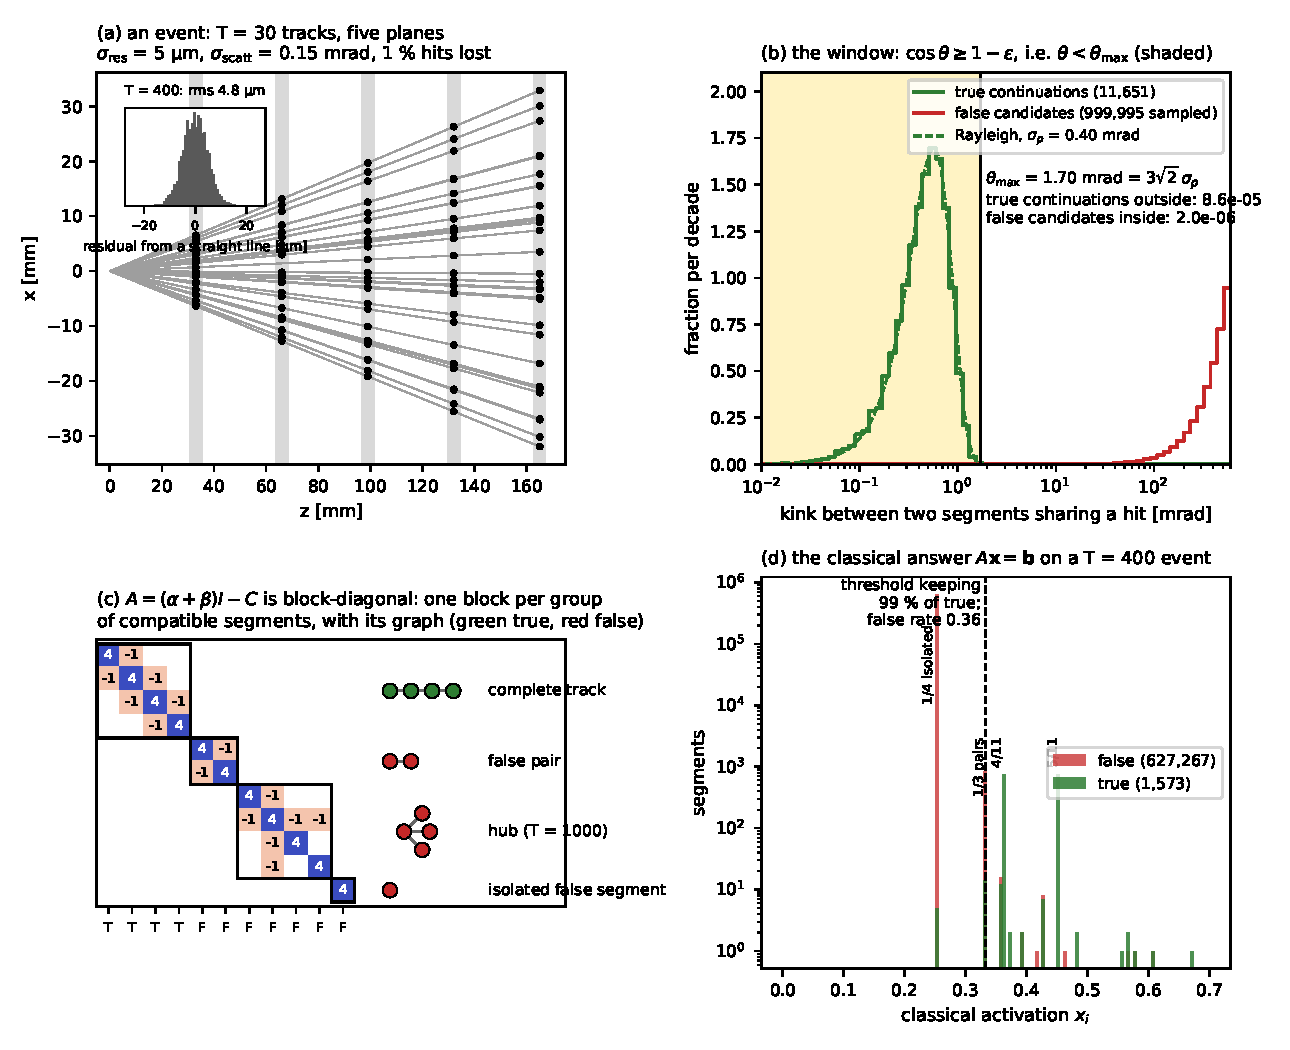
\includegraphics[width=\textwidth]{fig1_hits_to_hamiltonian.pdf}
\caption{\textbf{From hits to a Hamiltonian.} (a)~An event with $T=30$ tracks; inset, hit
residuals, the distance in $x$ between each hit and the straight line fitted through the hits of its
track, \js{what is this?} \gs{The hit residual is the distance in $x$ between a hit and the straight line fitted through all hits of its track. Its spread measures the resolution. I will define it in the caption.  } on a 400-track event. (b)~Kinks between segments that share a
hit: true continuations follow the Rayleigh law of width $\sigma_p$; false candidates lie far
outside the window $\theta<\theta_{\max}$ (shaded). (c)~Real blocks of $A=(\alpha+\beta)I-C$ and their graphs: a
complete track, a false pair, a hub and an isolated false segment. (d)~Classical activations on
a 400-track event with the threshold that keeps $99\%$ of true segments.}
\label{fig:hits}
\end{figure}

\paragraph{The one-bit filter.}
The one-bit filter (figure~\ref{fig:filters}a) prepares the uniform superposition over segments,
applies one bit of phase estimation to $e^{-iAt}$ with the phase bit $T$, sets the flag qubit $A$ when
$T$ reads zero, and uncomputes the phase bit. \gs{State, $|u\rangle$ and $p_i$ moved to Methods, section~\mbox{\ref{sec:m:onebit}}; marked for removal. The kept factors and false rates stay here.} \gsx{The $A=1$ part of the final state $|\Psi_4\rangle$ of
figure~\mbox{\ref{fig:filters}}a is} \js{$\cos(A)$ is not meaningful in this context. It is a probability, so it should be scalar. And what is $\mathbf{u}$? I need a bit more context to follow. Maybe we can write up the outcome of the 1-bit filter, which should be something like } \gs{Agreed, and I have rewritten this part. $|u\rangle$ is the uniform state over the $N$ candidate segments, $\mathbf{u}$ its vector of amplitudes $u_i=1/\sqrt N$. $p_i$ is a scalar: $[\cdot]_i$ takes component $i$ of the vector in the brackets. The state you wrote is not the state the circuit makes. After the first round, the phase bit $T$ holds $|0\rangle_T\otimes e^{-iAt/2}\cos(At/2)|u\rangle-i\,|1\rangle_T\otimes e^{-iAt/2}\sin(At/2)|u\rangle$. The flag $A$ is set to 1 on the $T=0$ part. The uncompute then gives the state in the equation below, and this state gives $p_i$. I will write the state after each stage of figure~\ref{fig:filters}a in Methods.}
\begin{gsxblock}
\begin{equation}
|1\rangle_A\otimes\Big[|0\rangle_T\otimes\cos^{2}\!\big(\tfrac{At}{2}\big)|u\rangle\;-\;\tfrac{i}{2}\,|1\rangle_T\otimes\sin(At)\,|u\rangle\Big],
\qquad |u\rangle=\frac{1}{\sqrt N}\sum_{i=1}^{N}|i\rangle ,
\end{equation}
\end{gsxblock}
\gsx{where $N$ is the number of candidate segments, so that after post-selection on $A=1$ the
probability of reading segment $i$ is}

\js{with $\psi = \frac 1 {2^n} \sum_{i=0}^{2^n-1} i$ and then continue from there? We could also clarify that $T = 2^n$ ?} \gs{The segment register has $n=\lceil\log_2 N\rceil$ qubits, with $N$ the number of candidate segments. $N$ is not a power of two in general. I will state $n$ at the register in figure~\ref{fig:filters}a and say in Methods how the unused basis states are treated.}
\begin{gsxblock}
\begin{equation}
p_i=\Big[\cos^{2}\!\big(\tfrac{At}{2}\big)\mathbf{u}\Big]_i^{2}+\Big[\tfrac12\sin(At)\,\mathbf{u}\Big]_i^{2},\qquad t=\frac{\pi}{\lambda_c},
\end{equation}
\end{gsxblock}
\js{Btw, this should be the probability when the ancilla is zero, but in the plot it says it should be one.} \gs{Both are correct. The circuit has two ancillas. The phase bit $T$ returns to 0. The flag $A$ is set to 1 when $T=0$ after the first round, and the post-selection reads $A=1$. The text now names both registers.}
\gsx{so the amplitude of every eigencomponent of the input is multiplied by $\cos(\lambda t/2)$} \js{should it not be the square?} \gs{The amplitude factor is $\cos(\lambda t/2)$. The probability weight is its square. The sentence now says `amplitude'.}\gsx{. With $t=\pi/\lambda_c$ the
zero lies at $\lambda=\lambda_c$,} \gss{The response of the one-bit filter has its zero at} the eigenvalue of every isolated segment \js{what about the $\sin$ contribution in $p_i$?} \gs{The sine term is the $T=1$ part of the same flagged state. Its amplitude on one eigencomponent is $\cos(\lambda t/2)\sin(\lambda t/2)$. It contains the factor $\cos(\lambda t/2)$, so it is also zero at $\lambda=\lambda_c$. The sum of the two terms on one eigencomponent is $\cos^2(\lambda t/2)$.}, and those segments are removed
exactly. Every other configuration keeps a factor fixed by where its eigenvalues lie
(figure~\ref{fig:filters}c): a false pair keeps $\KeptPair$, a false triple $\KeptTriple$, a
hub with three or five segments $\KeptHubThree$ or $\KeptHubFive$, and a complete track
$\KeptTrack$ on the eigenvalue that carries almost all of its weight. Every hub keeps more of
itself than a real track does. Holding $99\%$ of true segments, the filter's threshold must again fall to the level of the
broken tracks, and the false pairs, triples and hubs above them all survive: on the median event its
false rate matches the classical one, $\OneBitFarFourHundred$ at 400 tracks,
$\OneBitFarSevenHundred$ at 700 and $\OneBitFarThousand$ at 1000.

% Figure fig:filters moved to section sec:m:onebit (redundancy pass, 2026-10-27).
\gs{Figure~\mbox{\ref{fig:filters}} (circuits and one-bit response) moved to Methods, section~\mbox{\ref{sec:m:onebit}}.}

\paragraph{Segment classes kept by each solver.}
\gs{Class definitions moved to Methods, section~\mbox{\ref{sec:m:metrics}}; marked for removal. The counts and efficiencies stay here.} \gsx{We sort the segments into classes by the connected group they belong to. There are seven classes:
complete tracks; broken tracks, which lost a hit; contaminated tracks, which carry an accidental
false segment; isolated false segments; false pairs, two compatible false segments; false triples,
three compatible false segments in a chain; and hubs, where several compatible false segments share
one hit.}
Figure~\ref{fig:atlas} shows, at 1000 tracks and pooled over $\NEvents$ events, the value of
every segment of each class relative to each solver's threshold. The classical solver and the
one-bit filter, read at $99\%$ efficiency, keep all $\AtlasPairs$ false-pair segments and all
$\AtlasTriples$ false-triple segments. The degree-40 polynomial introduced in section~\ref{sec:r2}, read at the lowest threshold
with a false rate of at most $1\%$, keeps none of the false-pair segments, keeps
$\AtlasCompleteKeptQsvt$ of the $\AtlasComplete$ segments of complete tracks, and reaches an
efficiency of $\AtlasQsvtEff$ at a false rate of $\AtlasQsvtFar$. \gss{These two values are pooled over the $\NEvents$ events; the median over events is in table~\ref{tab:headline}.} The true segments it rejects
are the $\AtlasBrokenLostQsvt$ segments of broken tracks and $\AtlasContamLostQsvt$ segments of
contaminated tracks, whose eigenvalues differ from those of a complete track
(table~\ref{tab:headline}). Read at the same false rate of at most $1\%$, the classical solver
is close to the polynomial up to 400 tracks, but keeps $\ClassEffAtOneSevenHundred$ of true
segments at 700 and $\ClassEffAtOneThousand$ at 1000, and the one-bit filter keeps
$\OneBitEffAtOneFourHundred$ from 400 tracks upwards.

\begin{figure}[H]
\centering
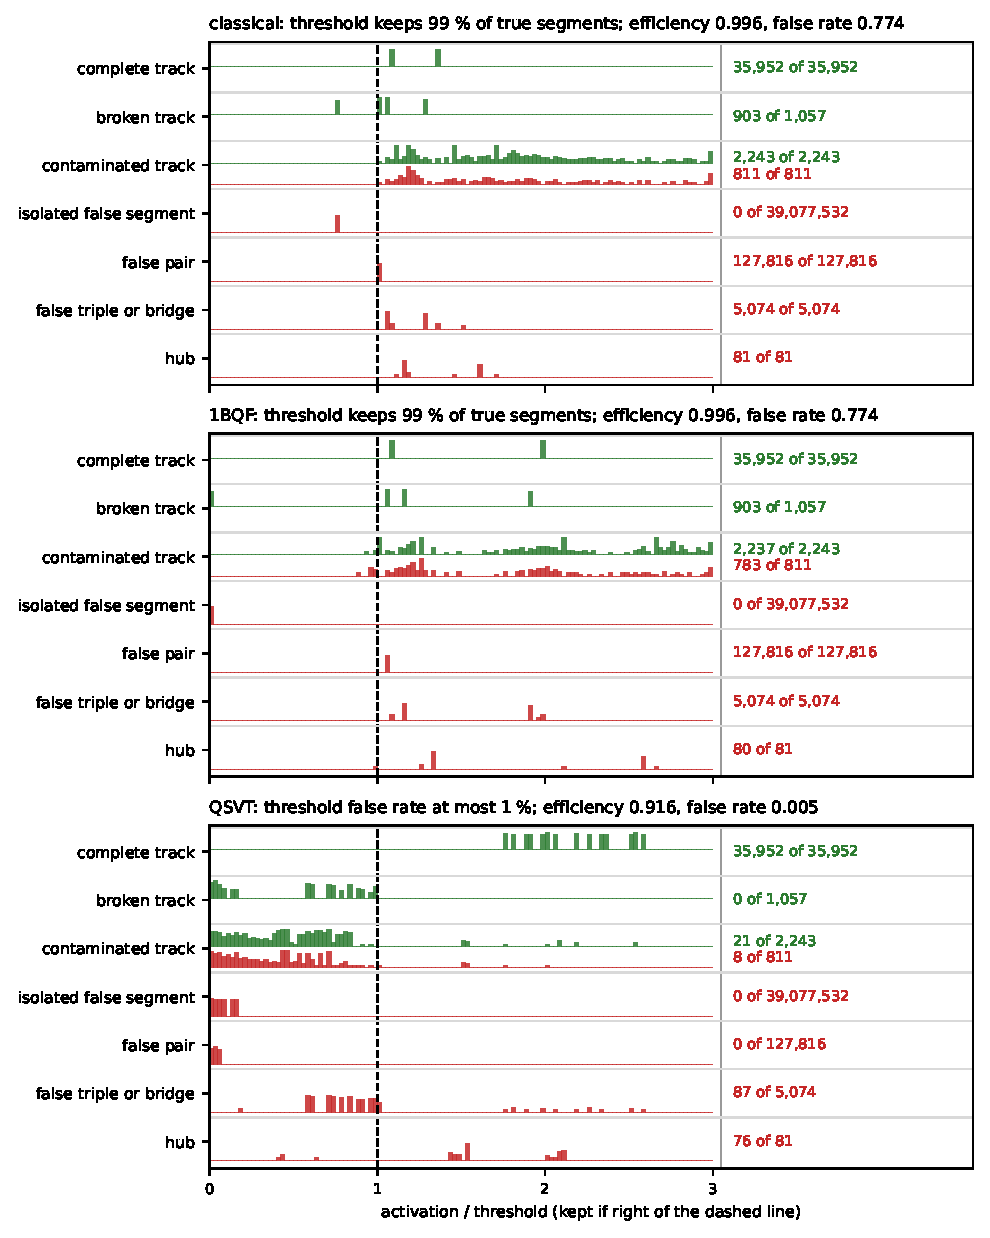
\includegraphics[width=0.92\textwidth]{fig3_error_atlas_T1000_with_qsvt.pdf}
\caption{\textbf{Segment classes kept by each solver}, at 1000 tracks pooled over
$\NEvents$ events. Activations are divided by each solver's threshold, so a segment is kept
when it lies to the right of the dashed line. Green, true segments; red, false; the kept
counts are given on the right. Classical solver and one-bit filter: threshold keeping $99\%$ of
true segments. Polynomial: lowest threshold with a false rate of at most $1\%$ \js{how is false rate defined? Because for the classical solver, it filters out nearly 40,000,000 tracks, right?} \gs{The false rate is the number of false segments kept divided by the number of all segments kept. It is one minus the purity. It is not the fraction of the 39 million candidates that leak. I will define it at the first use.  }. The same figure at 400 tracks is in the supplement\gss{ (figure~\ref{fig:atlas400})}. \js{what is classical solver? Can you give a reference please?} \gs{The classical solver is the direct solution of $A\mathbf{x}=\mathbf{b}$, read at a threshold on $x_i$, as in refs.~\cite{nicotra2023,trackhhl}. I will define it and cite it at the first use.  }}
\label{fig:atlas}
\end{figure}

\begin{table}[H]
\centering\small
\caption{Segment false rate at $99\%$ efficiency (top) and efficiency at a false rate of at most $1\%$
(bottom) for the three solvers, as medians over $\NEvents$ events (lowest event in brackets for the
polynomial). The polynomial reaches $99\%$ efficiency only when its threshold falls to the level of the
broken tracks, which is also the level of the rejected false segments, so its false rate at that point
is high; it is read at
the bottom working point throughout. \js{Why is the line between two efficiencies? And why is there no polynomial: false rate at 99\% efficiency? } \gs{The line separates the working points I use (first three rows) from the two cross-check rows. I will replace it by a clearer layout. The missing row exists: the median false rate of the polynomial at $99\%$ efficiency is $0.56$ at 200 tracks, $0.36$ at 400, $1.00$ at 700 and $1.00$ at 1000. To keep $99\%$ of true segments the threshold must reach the broken tracks, and the rejected population lies at the same level. I will add this row and this sentence.  }}
\label{tab:headline}
\begin{tabular}{lcccc}\toprule
 & $T=200$ & $T=400$ & $T=700$ & $T=1000$\\\midrule
\multicolumn{5}{l}{\textit{False rate at $99\%$ efficiency}}\\
Classical & $\ClassFarTwoHundred$ & $\ClassFarFourHundred$ & $\ClassFarSevenHundred$ & $\ClassFarThousand$\\
One-bit filter & $\OneBitFarTwoHundred$ & $\OneBitFarFourHundred$ & $\OneBitFarSevenHundred$ & $\OneBitFarThousand$\\
Polynomial & $\QsvtFarTwoHundred$ & $\QsvtFarFourHundred$ & $\QsvtFarSevenHundred$ & $\QsvtFarThousand$\\
\midrule
\multicolumn{5}{l}{\textit{Efficiency at a false rate of at most $1\%$}}\\
Classical & $\ClassEffAtOneTwoHundred$ & $\ClassEffAtOneFourHundred$ & $\ClassEffAtOneSevenHundred$ & $\ClassEffAtOneThousand$\\
One-bit filter & $\OneBitEffAtOneTwoHundred$ & $\OneBitEffAtOneFourHundred$ & $\OneBitEffAtOneSevenHundred$ & $\OneBitEffAtOneThousand$\\
Polynomial & $\QsvtEffTwoHundred$ ($\QsvtEffMinTwoHundred$) & $\QsvtEffFourHundred$ ($\QsvtEffMinFourHundred$) & $\QsvtEffSevenHundred$ ($\QsvtEffMinSevenHundred$) & $\QsvtEffThousand$ ($\QsvtEffMinThousand$)\\\bottomrule
\end{tabular}
\end{table}

\paragraph{A response with several zeros. \js{not a very scientific title} \gs{I will rename the paragraph `A response with more than one zero'.  }} Every segment class in figure~\ref{fig:atlas} sits on eigenvalues that are fixed by its graph, so
separating them does not need a different primitive, only a response with more than one zero.
The quantum singular value transformation provides it: $d$ calls to a block encoding of $A$,
with a phase rotation between calls, apply any polynomial of degree $d$ bounded by 1 on $[-1,1]$
(figure~\ref{fig:filters}b). Section~\ref{sec:r2} shows where the eigenvalues of each kind lie,
what the transformation is, and which polynomial we apply; section~\ref{sec:r3} measures it against
track multiplicity.

%==============================================================================================
\subsection{The problem as a spectrum, and a polynomial that separates it}\label{sec:r2}

\paragraph{\gsx{Every block has a spectrum fixed by its graph.}}
\js{I think that this should come prior to here} \gs{Agreed, see my reply at the Hamiltonian paragraph. This paragraph moves to section~\ref{sec:r1}.}
\gs{This paragraph and the next one are now in section~\mbox{\ref{sec:r1}}, with the derivation of the classical values; marked for removal here.}
\gsx{Because $A=\lambda_cI-C$ is block-diagonal, its eigenvalues are those of the individual blocks, and
on a block of $m$ segments with compatibility graph $G$ they are}
\begin{gsxblock}
\begin{equation*}
\lambda=\lambda_c-\mu,\qquad \mu\in\operatorname{spec}\big(C_G\big),
\end{equation*}
\end{gsxblock}
\gsx{where $C_G$ is the adjacency matrix of $G$. The graphs that occur are small and their spectra are
known in closed form. A chain of $m$ segments, which is what a complete track ($m=4$) or a broken
track ($m\le3$) is, has}
\begin{gsxblock}
\begin{equation*}
\lambda_k=\lambda_c-2\cos\!\Big(\frac{k\pi}{m+1}\Big),\qquad k=1,\dots,m ,
\end{equation*}
\end{gsxblock}
\gsx{so a complete track has exactly four eigenvalues, $\{2.382,\,3.382,\,4.618,\,5.618\}$ at
$\lambda_c=4$. We call these fixed eigenvalues the lines of the spectrum. An isolated segment has the single eigenvalue $\lambda_c$; a pair of compatible
segments has $\lambda_c\mp1$; a triple has $\lambda_c$ and $\lambda_c\mp\sqrt2$; and a hub, in which
$m$ segments leave or enter one hit, has $\lambda_c\pm\sqrt m$ together with $m-1$ copies of
$\lambda_c$. None of these depends on the event: detector geometry fixes the graph of a complete
track, and hence its four lines, for every track in every event.}

\paragraph{\gsx{Only some lines carry weight.}}
\gsx{The solution to \mbox{\eqref{eq:Axb}} on a block is a sum over its eigenvectors $\mathbf{v}_k$,}
\begin{gsxblock}
\begin{equation*}
\mathbf{x}\big|_{\rm block}=\sum_k\frac{\langle\mathbf{v}_k,\mathbf{b}\rangle}{\lambda_k}\,\mathbf{v}_k ,
\end{equation*}
\end{gsxblock}
\gsx{and the uniform input $\mathbf{b}=\beta\mathbf{1}$ reaches only the modes that are symmetric under
every relabelling of the block that leaves its graph unchanged; every other mode has
$\langle\mathbf{v}_k,\mathbf{b}\rangle=0$ exactly} \js{I do not understand this} \gs{The input $\mathbf{b}=\beta\mathbf{1}$ is the same on every segment. A relabelling of the segments that keeps the graph is a permutation $P$ with $PCP^{\mathsf T}=C$ and $P\mathbf{1}=\mathbf{1}$. For an eigenvector with $P\mathbf{v}=-\mathbf{v}$ I get $\langle\mathbf{v},\mathbf{1}\rangle=\langle P\mathbf{v},P\mathbf{1}\rangle=-\langle\mathbf{v},\mathbf{1}\rangle$, so the overlap is zero. For the chain, $P$ is the reflection and the modes $v_j=\sin(kj\pi/(m+1))$ with even $k$ are antisymmetric. I will add this argument.} \gsx{. We call a mode bright when that overlap is non-zero and
dark when it vanishes. A dark mode is in the spectrum of the block, but the input has no component along it} \js{??} \gs{Meaning: the eigenvalue is in the spectrum of the block, but the input vector has zero component along that eigenvector. A function $g(A)$ multiplies each eigencomponent by the scalar $g(\lambda_k)$, so a zero component stays zero. I will rewrite the sentence.  } \gsx{, and a function of $A$ multiplies each component by a scalar, so no function of $A$ applied to
$\mathbf{b}$ can give it one. For a chain the reflection $j\mapsto m+1-j$ is the only such
relabelling, so its antisymmetric modes are dark: a complete track is bright only on $2.382$ and
$4.618$, and carries $\TrackInputWeightLow\%$ of its input weight on the first
($\TrackSolutionWeightLow\%$ of its solution). A pair is bright only on $\lambda_c-1$, a triple on
$\lambda_c\mp\sqrt2$, and a hub of any size only on $\lambda_c\pm\sqrt m$.} \js{I would need more explanation on this whole paragraph I guess.} \gs{I will expand this paragraph with the argument above and with the explicit chain eigenvectors. (Done in this version: the expanded text is now in section~\mbox{\ref{sec:r1}}.)}

\paragraph{The measured spectrum.}
Figure~\ref{fig:spectrum}a shows where the input weight lies on the set of events at 1000 tracks,
split by segment class. Complete tracks put all of their weight on their two bright lines, and
$\NIsolatedThousand$ isolated segments sit exactly at $\lambda_c$. The false pairs lie on
$\lambda_c-1=3$, the false triples on $\lambda_c\mp\sqrt2$, and the broken tracks on the lines of
their shorter chains; all of them lie between the true lines, not on them. Two kinds are harder.
A hub with three segments has its bright line at $\lambda_c-\sqrt3=2.268$, only $0.11$ from the
track line at $2.382$, and $\HubNearTrue\%$ of the hubs' weight falls within $0.18$ of a bright true
line. A contaminated track, a real track that carries an accidental false segment, is no longer a
chain: its graph is a tree, its lines move, and only $\ContamNearTrue\%$ of its weight stays near
the true lines. These two kinds set the limits of every filter that acts on the spectrum alone.

\paragraph{The one-bit filter, read on the spectrum.}
Figure~\ref{fig:spectrum}b places the one-bit response $|\cos(\lambda t/2)|$ on the same axis. Its
single zero lies on the line that carries the most segments, $\lambda_c$, and removes them. On every
other line its factor is set by the distance from $\lambda_c$ alone, which is why the false pair at
$\lambda_c-1$ keeps $\KeptPair$, less than the track line at $2.382$ ($\KeptTrack$) only because it is
closer to the zero, and why the hub line at $2.268$, further from the zero than the track line,
keeps more ($\KeptHubThree$). A single cosine cannot be low on $3$ and high on $2.382$ without also
being high on $2.268$ and $2.586$: its shape is fixed, and only its zero can be placed.

\begin{figure}[H]
\centering
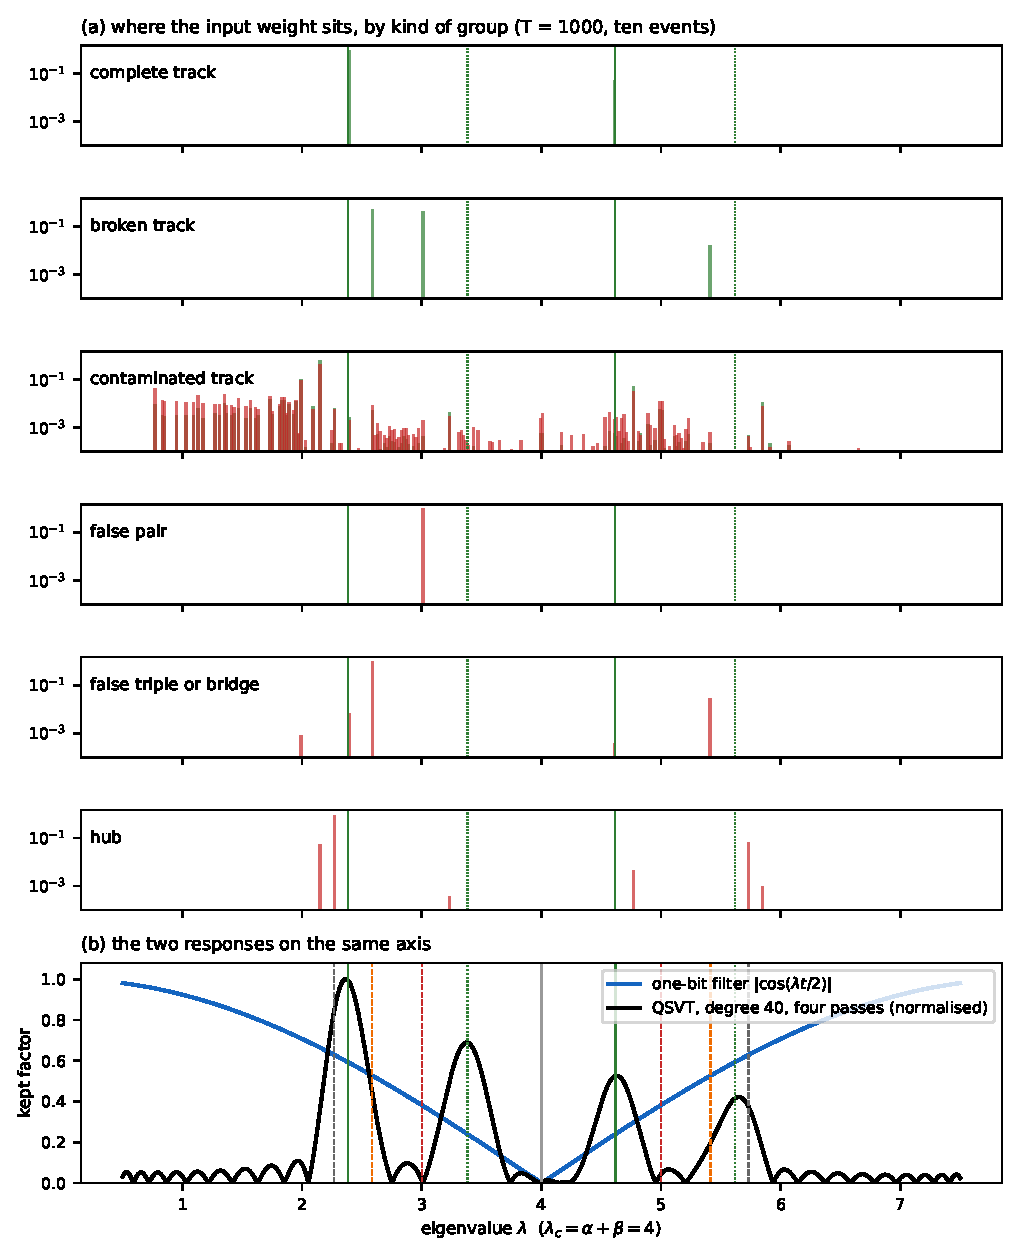
\includegraphics[width=0.92\textwidth]{fig4_spectrum.pdf}
\caption{\textbf{The problem as a spectrum.} (a)~Bright weight $\langle\mathbf{v}_k,\mathbf{1}\rangle^2$ of
every eigenmode, by segment class, on ten events with 1000 tracks; green, weight on true segments;
red, on false segments; each lane normalised to its total. The isolated segments, all at
$\lambda_c=4$, are not drawn. Vertical lines: the four lines of a complete track (solid, bright;
dotted, dark). (b)~The one-bit filter $|\cos(\lambda t/2)|$ and the QSVT polynomial (degree 40, four
passes, one on each line of a complete track, \js{passes = ?} \gs{A pass is an interval of the eigenvalue axis where the response is near its maximum. The target function has one pass on each of the four lines of a complete track. I will define `pass' at its first use in section~\ref{sec:r2}.  }, normalised to its maximum) on the same axis; dashed lines mark the pair ($\lambda_c\mp1$,
red), triple ($\lambda_c\mp\sqrt2$, orange) and three-segment hub ($\lambda_c\pm\sqrt3$, grey)
eigenvalues.}
\label{fig:spectrum}
\end{figure}

\paragraph{Block encodings and the quantum singular value transformation.}
A quantum circuit cannot apply $A$ directly, because $A$ is not unitary. It can apply a unitary $U$
that contains a rescaled copy of $A$ in one corner. With $X=(A-c_0I)/c_1$, where $c_0$ and $c_1$ are the centre and the half-width of the fit interval
defined below, \js{How do we choose $c_0$ and $c_1$? We should shortly comment on that I guess already here.} \gs{$c_0$ is the centre and $c_1$ the half-width of the fit interval $[\lambda_{\min}-\Delta,\lambda_{\max}+\Delta]$ of the paragraph on the polynomial. $\lambda_{\min}$ and $\lambda_{\max}$ are the extreme eigenvalues of the event, computed by the Lanczos method. I will define $c_0$ and $c_1$ here.  } so that the spectrum
of $X$ lies in $[-1,1]$, a block encoding of $X$ is a unitary on the segment register and one or more
ancilla qubits with
\begin{equation}
\big(\langle0|\otimes I\big)\,U\,\big(|0\rangle\otimes I\big)=X .
\end{equation}
The simplest one, used in figure~\ref{fig:filters}b and in our simulations, is the dilation
\begin{equation}
U=\begin{pmatrix}X&\sqrt{I-X^2}\\ \sqrt{I-X^2}&-X\end{pmatrix},
\end{equation}
which needs a single ancilla \js{Not sure this is needed here already. The paper is heavy enough as it is.} \gs{Agreed. I will remove the forward reference and keep the hit-priced block encoding for section~\ref{sec:r5} only.  }. The quantum singular value
transformation~\cite{gslw2019,martyn2021} then states that for every real polynomial $p$ of degree
$d$ with definite parity and $|p(x)|\le1$ on $[-1,1]$ there exist phases $\phi_0,\dots,\phi_d$ such
that the circuit
\begin{equation}
U_\Phi=e^{i\phi_0(2\Pi-I)}\prod_{k=1}^{d}\Big[U^{(\dagger)}\,e^{i\phi_k(2\Pi-I)}\Big],\qquad \Pi=|0\rangle\langle0|\otimes I,
\end{equation}
with $U$ and $U^\dagger$ alternating, has in the same corner a polynomial $P(X)$ whose real part is
$p(X)$. It makes $d$ calls in total, to $U$ and $U^\dagger$ in alternation, \js{Should this not be $U$ and $U^\dagger$ in total $d$ times?} \gs{Yes. Corrected: the sequence makes $d$ calls in total, to $U$ and $U^\dagger$ in alternation.}
and adds one signal qubit for the phases, and the phases are computed classically once for a given
$p$~\cite{dong2021}. A polynomial without definite parity is split into its even and odd parts, each
realised by its own phase sequence and combined with one further ancilla; the real part of the
complex polynomial the sequence produces is selected the same way. Measuring the ancillas in
$|0\rangle$ leaves the segment register in the state $p(X)|u\rangle/\lVert p(X)|u\rangle\rVert$, with
probability $\lVert p(X)|u\rangle\rVert^2$ up to a constant factor from the ancillas that select the
real part and combine the parities, where $|u\rangle$ is the uniform superposition over segments. Equivalently, since $\langle0|W^k|0\rangle=T_k(X)$ for the qubitised walk $W=(Z\otimes I)U$
built from the dilation~\cite{lowchuang2019}, a polynomial written as a Chebyshev series
$p(X)=\sum_kc_kT_k(X)$ can be applied as a linear combination of walk powers~\cite{childs2012}, at the
price of $\lceil\log_2(d+1)\rceil$ index qubits and a success probability reduced by
$(\sum_k|c_k|)^2$. Both routes apply the same polynomial; which is cheaper is the subject of
section~\ref{sec:r4}.

\paragraph{The one-bit filter is the degree-one case.}
The one-bit filter uses no block encoding: it calls the controlled evolution $e^{-iAt}$ directly.
The same polynomial construction applies to controlled evolutions~\cite{dong2022}, with the
variable $u=\cos(\lambda t/2)$ in place of $x$: a sequence of $d$ controlled evolutions with phase
rotations between them applies polynomials of degree $d$ in $u$ bounded by 1 on $[-1,1]$, subject to the same parity
conditions. The one-bit
interferometer is the shortest such sequence, and the response it applies, $\cos(\lambda t/2)$, is
the polynomial $p(u)=u$: degree one, one root. Every further call adds one degree, and with it one further pass, an interval of the eigenvalue
axis on which the response is near its maximum, or one further stop band, an interval on which it is
near zero, that can be placed on the spectrum. \js{I think that this paragraph is very important, so it deserves a bit more details, right? Can we see directly from Fig. 2a and b that the statement is true? Or can we compute it based on the exact representation of the final result of the algorithms?} \gs{Yes, I can compute it from the circuit. In figure~\ref{fig:filters}a the two Hadamard gates around the controlled $e^{-iAt}$ give, on the $T=0$ part, $\tfrac12(I+e^{-iAt})=e^{-iAt/2}\cos(At/2)$. This is a block encoding of $\cos(At/2)$ up to a phase. It is the degree-one case of the construction of ref.~\cite{dong2022}, with the controlled evolution in place of $U$. Figure~\ref{fig:filters}b with $d=1$ and this $U$ is the same circuit. I will add this derivation to the paragraph.} 

\paragraph{The polynomial we apply.}
The spectrum of figure~\ref{fig:spectrum}a sets the requirement on the response: pass the lines of a
complete track and reject everything between them. We write this as a target function on the
eigenvalue axis,
\begin{equation}
g(\lambda)=\frac{1}{\lambda}\max_{k}\exp\!\Big[-\Big(\frac{\lambda-\lambda_k}{h}\Big)^2\Big],\qquad
\lambda_k=\lambda_c-2\cos\!\Big(\frac{k\pi}{5}\Big),
\end{equation}
a narrow pass on each true line, where $h$ is the half-width of each pass, \js{$h$ defined as ...?} \gs{$h$ is the half-width of each pass in eigenvalue units, $h=0.18$ throughout. The sentence will say `where $h$ is the half-width of each pass'.  } weighted by $1/\lambda$ so that on those lines
the response keeps the relative amplitudes of the classical solution. We fit $g$ by least squares
with a Chebyshev series of degree $d$ on the interval $[\lambda_{\min}-\Delta,\lambda_{\max}+\Delta]$,
where $\lambda_{\min}$ and $\lambda_{\max}$ are the extreme eigenvalues of the event, computed by the
Lanczos method, and
$\Delta=0.05(\lambda_{\max}-\lambda_{\min})+0.2$ a margin, and rescale the result so that
$|p|\le0.95$ on the fit interval $[\lambda_{\min}-\Delta,\lambda_{\max}+\Delta]$, the domain of the
block encoding \js{I guess you mean the interval from $\lambda_{\min}$ to $\lambda_{\max}$? Then specify it. } \gs{No, the fit interval $[\lambda_{\min}-\Delta,\lambda_{\max}+\Delta]$. The bound must hold on the full domain of the block encoding, and this domain is the fit interval. I will name it.  }. Throughout this paper $d=40$ and $h=0.18$, and we call this
polynomial the QSVT.

\paragraph{Choice of degree.}
A polynomial of degree $d$ has at most $d$ zeros, so on an interval of length $L$ the mean distance
between adjacent zeros is at least $L/d$; a pass or a stop band needs a zero on each side, so it cannot
be narrower than this distance \js{Is there a reason not to go with the full width? Then you save all these factors of two.} \gs{No reason. I will use the full width $L=2W$ and write the resolution as $L/d$.  } \js{This is so unspecific, that it is meaningless. What does 'features' mean? If you mean roots, then this makes sense} \gs{Agreed. A polynomial of degree $d$ has at most $d$ zeros, so the mean distance between adjacent zeros on an interval of length $L$ is at least $L/d$. A pass or a notch needs two zeros around it, so it cannot be narrower than this distance. I will write it in this way.  }. At 1000 tracks the fit interval is $[\DomainLow,\DomainHigh]$, of length $L=\DomainLength$, so
degree 40 resolves $\ResolutionForty$ and degree 60 resolves $\ResolutionSixty$. The closest false line the design aims to reject is the triple line at $2.586$, $0.20$ from the
track line at $2.382$, which degree 40 resolves with no margin; the three-segment hub line at $2.268$, $0.11$ away,
is beyond it. The resulting response (figure~\ref{fig:spectrum}b) keeps
$\QTrackLow$ of its maximum on the dominant track line and $\QTrackHigh$ on the second, and
$\QPairLow$ on the false pair line, against $\KeptPair$ for the one-bit filter: relative to the
track line, the false pairs, the largest coupled false population, are suppressed
$(\KeptPair/\KeptTrack)/(\QPairLow/\QTrackLow)=\PairSuppression$ \js{If I compute correctly, 0.38/0.014 = 27, so not 45. Or am I mistaken?} \gs{The ratio 27 is the absolute ratio of the two pair factors. The value 45 is relative to the track line, as the sentence says: $(\KeptPair/\KeptTrack)/(\QPairLow/\QTrackLow)=45.8$. I will write this formula in the text so that the reader can check it.  } times more strongly than by the one-bit filter. It keeps $\QIso$ on the isolated line, not zero, but a factor small enough that every
isolated segment lies far below every true track. It keeps $\QTripleLow$ on the triple line at $2.586$,
which lies on the slope of the track pass, and $\QHubLow$ on the hub line at $2.268$, which no
polynomial of this degree can separate from the track line $0.11$ away.

\paragraph{Number of passes.}
\js{Again, you should explain what you mean by passes!} \gs{See my reply at figure~\ref{fig:spectrum}. I will define `pass' in section~\ref{sec:r2} before this point.  }
A complete track is bright only on two of its four lines, so passes on the two dark lines may
appear unnecessary. We tested this on the simulated events of section~\ref{sec:r1} \js{Funny, but not scientifically ;-)} \gs{I will replace `directly on the corpus' by `on the simulated events of section~\ref{sec:r1}'.  } with $\TeethNDesigns$ designs (four passes or two
bright passes, degrees 24, 40 and 60, half-widths $0.12$ to $0.30$), choosing on five events and
measuring on the other five. Placing the passes on the two dark lines alone removes the selectivity of the filter:
efficiency at a false rate of at most $1\%$ falls to $\TeethDarkTwoHundred$ at 200 tracks and
below $0.001$ \js{Really exactly zero?} \gs{The median over the five held-out events is exactly zero. The largest value on one event is $0.0005$. I will write `below $0.001$ on every held-out event'.  } on every held-out event at 1000, a direct confirmation that the weight of a track is on its bright lines. At equal
degree and width, two bright passes and four passes give the same result within the event-to-event
spread ($\TeethBrightThousand$ against $\TeethFourThousand$ at 1000 tracks, degree 40); the
advantage that bright passes alone showed on noiseless events in our earlier study does not carry
over to these events. What does matter is resolution. Degree 60 with half-width $0.12$ raises the efficiency at 700 tracks from
$\TeethFourSeven$ to $\TeethFourSixtySeven$ with four passes and to $\TeethBestSeven$ with two, and at
1000 tracks to $\TeethFourSixtyThousand$ and $\TeethBestThousand$, at one and a half times the calls.
We keep degree 40 with four passes as the reference design and report the higher degree as a variant
in section~\ref{sec:r3}.

\paragraph{Reading the output.}
After post-selection the probability of reading segment $i$ is proportional to
$[p(A)\mathbf{b}]_i^2$, so the amplitude $|[p(A)\mathbf{b}]_i|$ plays the role that $x_i$ plays for
the classical solver. Its distribution is well separated: the segments of complete tracks lie well above every
segment the polynomial rejects, with broken tracks, contaminated tracks and false triples in
between (figure~\ref{fig:atlas}).
We therefore read the QSVT at the lowest threshold with a false rate of at most $1\%$ and report the
efficiency it keeps, while the classical solver and the one-bit filter, whose true and false levels overlap, are read at the threshold that keeps $99\%$ of true segments. In all our figures the QSVT
amplitudes are computed exactly, by applying $p$ to the eigenvalues of each block and checked
against the three-term Chebyshev recursion on the full sparse matrix; they are what any exact
implementation of the circuit produces after post-selection.

%==============================================================================================
\subsection{Results against track multiplicity}\label{sec:r3}

\paragraph{\gss{Segment-level metrics of each solver.}}
\gss{Figure~\ref{fig:segmetrics} gives the segment-level metrics of the three solvers against $T$, in the form of the one-bit filter paper~\cite{trackhhl}: the segment efficiency $\eff$, the segment false rate $\far$, the number of candidate segments and the number of false segments kept. A segment is active when its value exceeds the solver's threshold; no efficiency or false-rate level is imposed. The classical solver is read at the fixed threshold $x_i>\beta/\lambda_c+0.10=\SegClassTau$ of ref.~\cite{trackhhl}. The one-bit filter sends every isolated segment to zero, so it is read at a threshold just above zero; the QSVT is read in the same way, just above the level of its isolated segments. The number of false candidates grows as $T^2$ and the number of true segments as $T$. All three solvers keep about $99\%$ of the true segments at every $T$. The false rate of the classical solver rises to $\SegFarClassThousand$ at 1000 tracks; that of the one-bit filter to $\SegFarOneBitThousand$, because every false pair, triple and hub lies above zero; and that of the QSVT to $\SegFarQsvtThousand$ with a large spread between events, because the false pairs, suppressed to $1\%$ of the track level, still lie above the isolated level. Table~\ref{tab:segmetrics} gives the numbers.}

\begin{figure}[H]
\centering
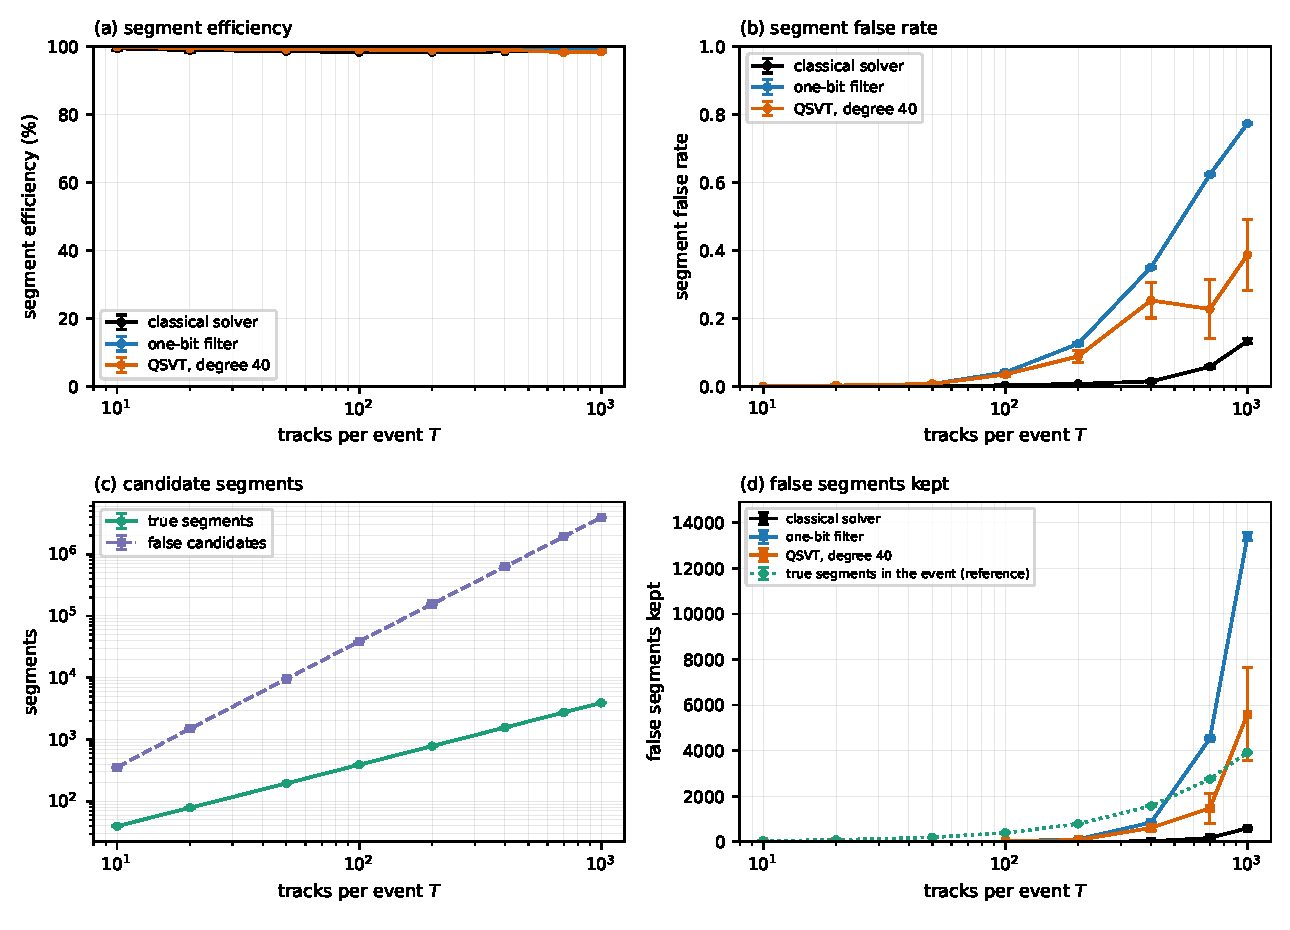
\includegraphics[width=\textwidth]{fig8_segment_metrics.pdf}
\caption{\gss{\textbf{Segment-level metrics against track multiplicity.} (a)~Segment efficiency and (b)~segment false rate of each solver: classical solver at the fixed threshold $\SegClassTau$, one-bit filter and QSVT (degree 40) at a threshold just above the level of their isolated segments. (c)~Candidate segments in the event, true and false. (d)~False segments kept by each solver, with the number of true segments in the event for reference. Points are means over the $\NEvents$ events and error bars the standard error of the mean.}}
\label{fig:segmetrics}
\end{figure}

\begin{table}[H]
\centering\footnotesize
\caption{\gss{\textbf{Segment-level metrics of each solver}, means over the $\NEvents$ events with the standard error of the mean: segment efficiency $\eff$, segment false rate $\far$ and the number of false segments kept, at the thresholds of figure~\ref{fig:segmetrics}.}}
\label{tab:segmetrics}
\begin{tabular}{rrrrrrrrrr}
\toprule
 & \multicolumn{3}{c}{Classical} & \multicolumn{3}{c}{One-bit filter} & \multicolumn{3}{c}{QSVT, degree 40}\\
\cmidrule(lr){2-4}\cmidrule(lr){5-7}\cmidrule(lr){8-10}
$T$ & $\varepsilon_{\rm seg}$ & $f_{\rm seg}$ & false kept & $\varepsilon_{\rm seg}$ & $f_{\rm seg}$ & false kept & $\varepsilon_{\rm seg}$ & $f_{\rm seg}$ & false kept\\\midrule
10 & 0.995 $\pm$ 0.005 & 0.000 $\pm$ 0.000 & 0 & 1.000 $\pm$ 0.000 & 0.000 $\pm$ 0.000 & 0 & 1.000 $\pm$ 0.000 & 0.000 $\pm$ 0.000 & 0\\
20 & 0.989 $\pm$ 0.006 & 0.000 $\pm$ 0.000 & 0 & 0.995 $\pm$ 0.004 & 0.002 $\pm$ 0.002 & 0 & 0.995 $\pm$ 0.004 & 0.002 $\pm$ 0.002 & 0\\
50 & 0.987 $\pm$ 0.002 & 0.000 $\pm$ 0.000 & 0 & 0.993 $\pm$ 0.002 & 0.007 $\pm$ 0.003 & 1 & 0.993 $\pm$ 0.002 & 0.007 $\pm$ 0.003 & 1\\
100 & 0.984 $\pm$ 0.002 & 0.003 $\pm$ 0.002 & 1 & 0.994 $\pm$ 0.001 & 0.041 $\pm$ 0.005 & 17 & 0.991 $\pm$ 0.002 & 0.035 $\pm$ 0.006 & 14\\
200 & 0.984 $\pm$ 0.002 & 0.007 $\pm$ 0.001 & 6 & 0.993 $\pm$ 0.001 & 0.125 $\pm$ 0.004 & 111 & 0.990 $\pm$ 0.001 & 0.088 $\pm$ 0.017 & 78\\
400 & 0.985 $\pm$ 0.001 & 0.015 $\pm$ 0.002 & 23 & 0.996 $\pm$ 0.001 & 0.351 $\pm$ 0.003 & 844 & 0.992 $\pm$ 0.003 & 0.253 $\pm$ 0.052 & 610\\
700 & 0.987 $\pm$ 0.001 & 0.057 $\pm$ 0.004 & 166 & 0.996 $\pm$ 0.001 & 0.623 $\pm$ 0.002 & 4{,}538 & 0.983 $\pm$ 0.003 & 0.228 $\pm$ 0.086 & 1{,}470\\
1000 & 0.986 $\pm$ 0.001 & 0.133 $\pm$ 0.007 & 596 & 0.996 $\pm$ 0.001 & 0.774 $\pm$ 0.002 & 13{,}378 & 0.985 $\pm$ 0.003 & 0.387 $\pm$ 0.105 & 5{,}596\\
\bottomrule
\end{tabular}

\end{table}

\paragraph{Efficiency at a false rate of at most $1\%$.}
Figure~\ref{fig:mult}a shows the efficiency of each solver at the lowest threshold with a false rate
of at most $1\%$, against $T$. The polynomial keeps $\QsvtEffTwoHundred$ of true segments at 200
tracks, $\QsvtEffFourHundred$ at 400, $\QsvtEffSevenHundred$ at 700 and $\QsvtEffThousand$ at 1000;
its lowest event at 1000 tracks keeps $\QsvtEffMinThousand$. The classical solver is within $0.02$
of the polynomial up to $\ClassCloseUpToT$ tracks. It falls to $\ClassEffAtOneSevenHundred$ at 700
and $\ClassEffAtOneThousand$ at 1000. The one-bit filter falls to $\OneBitEffAtOneFourHundred$ at
400 tracks and stays at $\OneBitPlateau$: a false rate of $1\%$ requires a threshold above the
level of the false pairs, and above that level only the two middle segments of each complete track
remain, since the end segments lie next to the false pairs. On single events the one-bit filter
reaches no threshold with a false rate of $1\%$ at all (the dots at zero).

\paragraph{False rate at $99\%$ efficiency.}
Figure~\ref{fig:mult}b shows the false rate at the threshold that keeps $99\%$ of true segments.
The classical solver and the one-bit filter give the same value on the median event:
$\ClassFarTwoHundred$ at 200 tracks, $\ClassFarFourHundred$ at 400, $\ClassFarSevenHundred$ at
700 and $\ClassFarThousand$ at 1000. The polynomial's false rate at $99\%$ efficiency is
$\QsvtFarSevenHundred$ at 700 tracks and $\QsvtFarThousand$ at 1000: the final one percent of true
segments belong to broken and contaminated tracks, and their level lies below the rejected population.
Below 400 tracks the polynomial's value differs strongly between events, because the threshold either remains
above that population or falls below it.

\paragraph{The full curves.}
Figure~\ref{fig:curves} shows efficiency against false rate for the three solvers at 200, 400, 700
and 1000 tracks, pooled over the ten events. \gs{The two struck sentences do not match the numbers; the teal sentences below replace them.} \gsx{The classical and one-bit curves coincide.} Both have a
step at an efficiency of $0.5$: the end segments of complete tracks and the false pairs share a
level. \gsx{From 400 tracks on, the polynomial's curve lies above both at every false rate below $10\%$.}
\gss{The classical and one-bit curves coincide at $99\%$ efficiency, but not at low false rate: at a false rate of $1\%$ the one-bit filter stays on the step at $0.5$ from 400 tracks on, while the classical solver keeps $\ClassEffAtOneFourHundred$ at 400 tracks. At 400 tracks the classical and polynomial curves meet at a false rate of $1\%$; from 700 tracks on, the polynomial's curve lies above both at every false rate below $10\%$ (table~\ref{tab:headline}).}

\paragraph{\gss{Other detector configurations.}}
\gss{We chose the configuration of this paper after a scan of four configurations, with $\ScanNEvents$ events at each multiplicity. Supplementary table~\ref{tab:scan} gives the result. At a resolution of $3\,\mu$m and of $5\,\mu$m, the polynomial keeps at least $\ScanQsvtFiveUmThousand$ of true segments at a false rate of at most $1\%$, up to 1000 tracks. At $10\,\mu$m and a kink of $0.30$\,mrad per plane, it keeps $\ScanQsvtTenUmFourHundred$ at 400 tracks and $\ScanQsvtTenUmSevenHundred$ at 700. At $15\,\mu$m and $0.45$\,mrad, it keeps $\ScanQsvtFifteenUmTwoHundred$ at 200 tracks and $\ScanQsvtFifteenUmThousand$ at 1000. The gain of the polynomial thus holds only while the acceptance window is narrow.}

\paragraph{Degree 60.}
A polynomial of degree 60 with half-width $0.12$, chosen on five events and read on the other five,
raises the efficiency at a false rate of at most $1\%$ from $\TeethFourSeven$ to
$\TeethFourSixtySeven$ at 700 tracks and from $\TeethFourThousand$ to $\TeethFourSixtyThousand$ at
1000, for one and a half times the calls (dashed line in figure~\ref{fig:mult}a).

\begin{figure}[H]
\centering
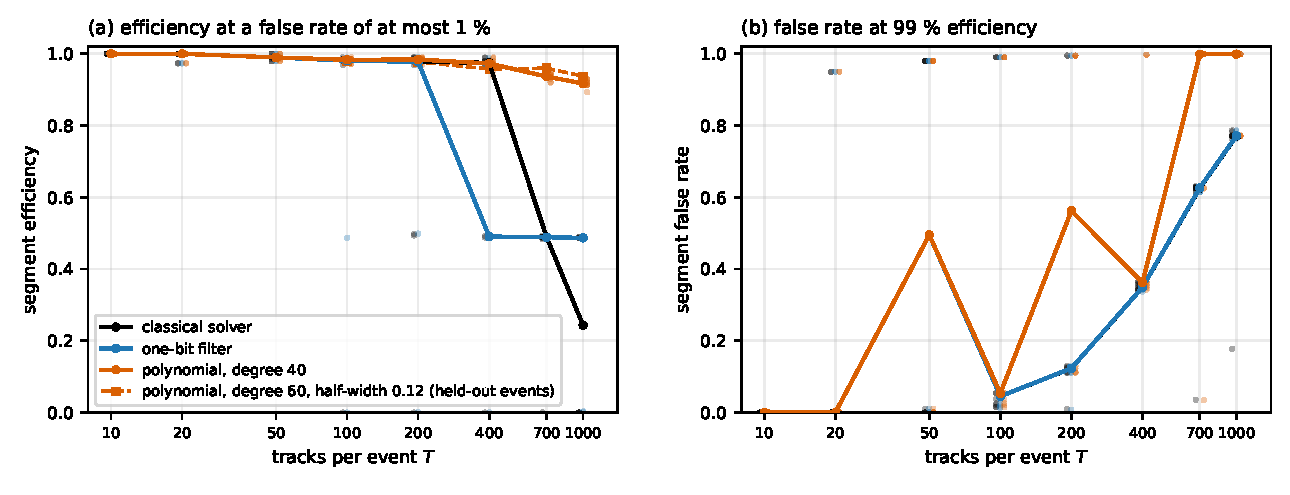
\includegraphics[width=\textwidth]{fig5_multiplicity.pdf}
\caption{\textbf{Results against track multiplicity.} (a)~Segment efficiency at the lowest
threshold with a false rate of at most $1\%$, against $T$, for the classical solver, the one-bit
filter and the polynomial (degree 40, four passes, half-width $0.18$). Lines are medians over the
$\NEvents$ events; dots are single events. Dashed: degree 60, half-width $0.12$, on the five
held-out events of the design scan. (b)~Segment false rate at the threshold that keeps $99\%$ of
true segments, same solvers.}
\label{fig:mult}
\end{figure}

\begin{figure}[H]
\centering
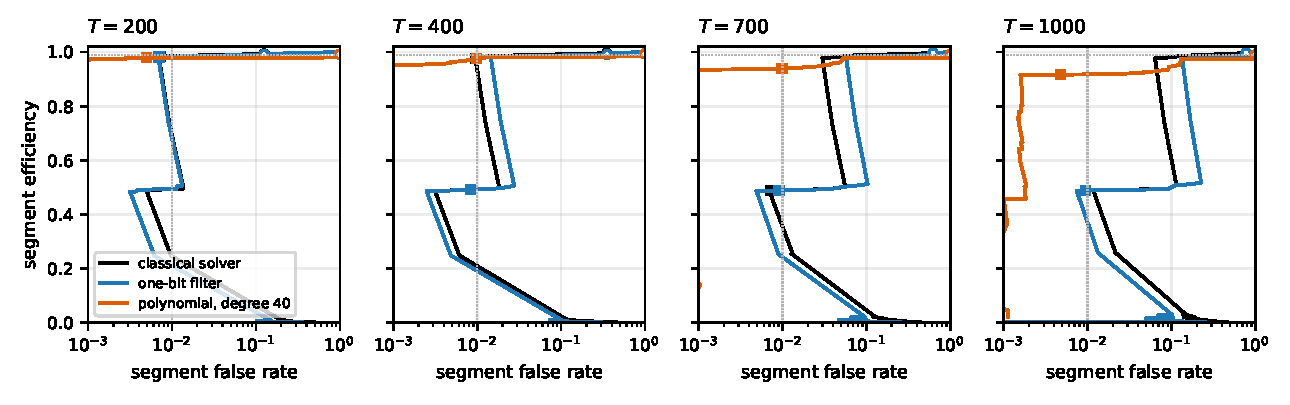
\includegraphics[width=\textwidth]{fig6_curves.pdf}
\caption{\textbf{Efficiency against false rate.} Segment efficiency against segment false rate at
200, 400, 700 and 1000 tracks, pooled over the $\NEvents$ events, for the three solvers. Open
circles: the threshold that keeps $99\%$ of true segments. Squares: the lowest threshold with a false
rate of at most $1\%$. Dotted lines: $99\%$ efficiency and $1\%$ false rate.}
\label{fig:curves}
\end{figure}

\subsection{Computational cost}\label{sec:r4}

\paragraph{One currency.}
We price every algorithm in two-qubit gates per solved event: calls per shot, times the
amplification rounds $\pi/(4\sqrt P)$ that raise the post-selection probability $P$ to order one,
times the two-qubit gates per call. A shot is one run of the circuit up to its measurement. A route is one circuit that applies the
same filter. The width is counted separately. Table~\ref{tab:cost} gives the
factors at 400 and 1000 tracks; figure~\ref{fig:cost} gives them against $T$.

\paragraph{Width.}
The segment register has $\lceil\log_2 4T^2\rceil$ qubits: $\NSysFourHundred$ at 400 tracks and
$\NSysThousand$ at 1000. The one-bit filter adds two ancillas, the phase sequence four, the
Chebyshev walk seven, and eight-bit HHL nine. At 1000 tracks the four routes need
$\WidthOneBitThousand$, $\WidthPhaseThousand$, $\WidthWalkThousand$ and $\WidthHhlThousand$ logical
qubits.

\paragraph{Calls per shot.}
The number of calls to the primitive per shot does not depend on $T$. The one-bit filter makes
$\CallsOneBit$. The phase sequence makes $\CallsPhase$: the degree-40 polynomial has no definite
parity, so its even and odd parts are applied by separate sequences, and the real part of each is
selected by a second run. The Chebyshev walk makes $\CallsWalk$ for the 41 terms of the series.
Eight-bit HHL makes $\CallsHhl$.

\paragraph{Gates per call.}
The controlled evolution $e^{-iAt}$ was transpiled to two-qubit gates up to $\MeasuredTMax$ tracks
and follows $\CxEvoPrefactor\,T^{\CxEvoExponent}$: $\CxEvoFourHundred$ gates per call at 400 tracks
(measured) and $\CxEvoThousand$ at 1000 (extrapolated). A block encoding priced by detector hits
(section~\ref{sec:r5}) is modelled at $\CxHitPrefactor\,T^{\CxHitExponent}$: $\CxHitFourHundred$
gates per call at 400 tracks and $\CxHitThousand$ at 1000.

\paragraph{Amplification.}
The post-selection probability is measured on the set of events. For the polynomial it is
$\PPhaseFourHundred$ at 400 tracks and $\PPhaseThousand$ at 1000, and follows
$\PPhasePrefactor\,T^{-\PPhaseExponent}$ above 100 tracks; for the one-bit filter it is
$\POneBitThousand$ at 1000 tracks. The walk divides the polynomial's probability by the squared
one-norm of its Chebyshev coefficients. Amplitude amplification raises each to order one in
$\pi/(4\sqrt P)$ rounds: $\RoundsPhaseThousand$ for the polynomial at 1000 tracks.

\paragraph{Totals.}
At 1000 tracks the phase sequence costs $\GatesEvoPhaseThousand$ two-qubit gates per event with the
controlled evolution and $\GatesHitPhaseThousand$ with the hit-priced encoding. The Chebyshev walk
costs $\GatesEvoWalkThousand$ and $\GatesHitWalkThousand$ for three more qubits, and costs fewer gates. The one-bit filter costs $\GatesEvoOneBitThousand$ and $\GatesHitOneBitThousand$.
Eight-bit HHL costs $\GatesEvoHhlThousand$ as a structure-level estimate, at the level of the walk:
the polynomial makes many fewer calls per shot than HHL, but its post-selection probability is two to
three orders of magnitude smaller, and amplification cancels the difference. The one-bit filter
costs thirty times fewer gates than the walk. Reading the kept segments after amplification needs of order
$4T\ln(4T)$ post-selected samples.

\textit{[Classical loading of the hit oracle, $0.4$\,ms and 8\,KB at 400 tracks (chapter 11.6):
to be re-derived on the corpus and ledgered before it is quoted.]}

\begin{table}[H]
\centering\footnotesize
\caption{\textbf{Cost at 400 and 1000 tracks.} Logical qubits, calls per shot, post-selection
probability $P$ (measured on the set of events; HHL from the resource model), amplified calls per event
$\lceil$calls$\times\pi/(4\sqrt P)\rceil$, and two-qubit gates per event with the controlled
evolution (measured at 400 tracks, extrapolated at 1000) and with the hit-priced block encoding
(model). Entries are given as 400 / 1000 tracks.}
\label{tab:cost}
\resizebox{\textwidth}{!}{%
\begin{tabular}{lcccccc}\toprule
Route & qubits & calls per shot & $P$ & amplified calls & gates, evolution & gates, hit-priced\\\midrule
One-bit filter & $\WidthOneBitFourHundred$ / $\WidthOneBitThousand$ & $\CallsOneBit$ & $\POneBitFourHundred$ / $\POneBitThousand$ & $\TotalCallsOneBitFourHundred$ / $\TotalCallsOneBitThousand$ & $\GatesEvoOneBitFourHundred$ / $\GatesEvoOneBitThousand$ & $\GatesHitOneBitFourHundred$ / $\GatesHitOneBitThousand$\\
QSVT, phase sequence & $\WidthPhaseFourHundred$ / $\WidthPhaseThousand$ & $\CallsPhase$ & $\PPhaseFourHundred$ / $\PPhaseThousand$ & $\TotalCallsPhaseFourHundred$ / $\TotalCallsPhaseThousand$ & $\GatesEvoPhaseFourHundred$ / $\GatesEvoPhaseThousand$ & $\GatesHitPhaseFourHundred$ / $\GatesHitPhaseThousand$\\
QSVT, Chebyshev walk & $\WidthWalkFourHundred$ / $\WidthWalkThousand$ & $\CallsWalk$ & $\PWalkFourHundred$ / $\PWalkThousand$ & $\TotalCallsWalkFourHundred$ / $\TotalCallsWalkThousand$ & $\GatesEvoWalkFourHundred$ / $\GatesEvoWalkThousand$ & $\GatesHitWalkFourHundred$ / $\GatesHitWalkThousand$\\
HHL, eight bits (estimate) & $\WidthHhlFourHundred$ / $\WidthHhlThousand$ & $\CallsHhl$ & $\PHhlFourHundred$ / $\PHhlThousand$ & $\TotalCallsHhlFourHundred$ / $\TotalCallsHhlThousand$ & $\GatesEvoHhlFourHundred$ / $\GatesEvoHhlThousand$ & $\GatesHitHhlFourHundred$ / $\GatesHitHhlThousand$\\\bottomrule
\end{tabular}}
\end{table}

\begin{figure}[H]
\centering
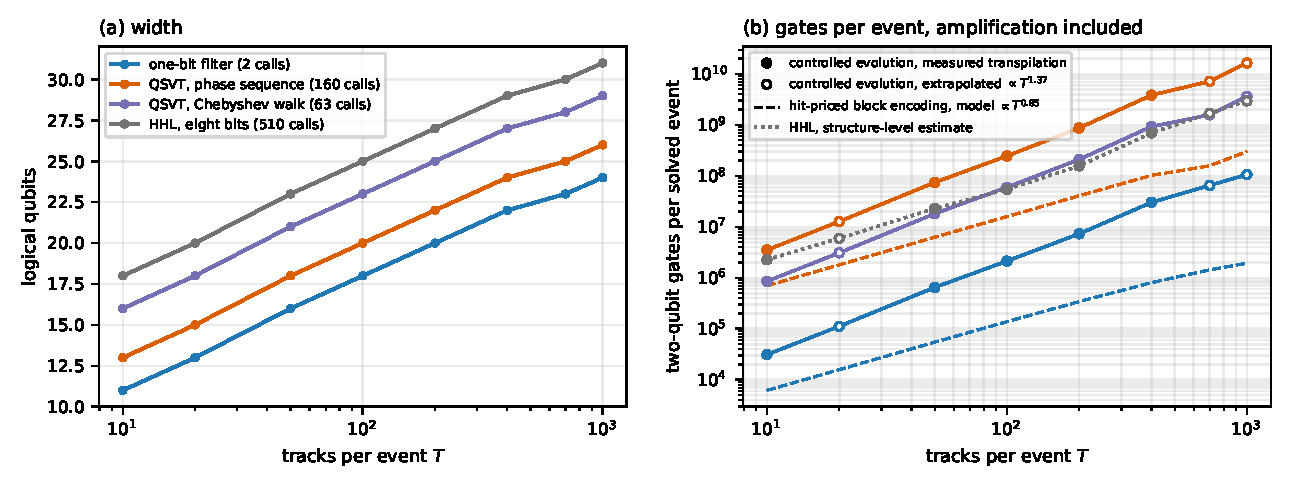
\includegraphics[width=\textwidth]{fig7_cost.pdf}
\caption{\textbf{Cost against track multiplicity.} (a)~Logical qubits: the segment register
$\lceil\log_2 4T^2\rceil$ plus the ancillas of each route. (b)~Two-qubit gates per solved event,
amplification included. Filled markers: the controlled evolution priced by its measured
transpilation. Open markers: its power-law extrapolation. Dashed: the hit-priced block encoding, a
model. Dotted: HHL, a structure-level estimate.}
\label{fig:cost}
\end{figure}

\subsection{A block encoding priced by detector hits}\label{sec:r5}
\textit{[Scope decision pending: the cost model below, or the full construction.]}

The dilation of section~\ref{sec:r2} prices each call by the entries of $A$. A block encoding can
instead price each call by the hits: the matrix is not stored, and each call reads the hit
positions and computes the compatibility of two segments at each call. The cost model gives
$\CxHitPrefactor\,T^{\CxHitExponent}$ two-qubit gates per call, $\CxHitFourHundred$ at 400 tracks
against $\CxEvoFourHundred$ for the controlled evolution, for $\HitOracleAncillas$ workspace qubits
over the register. The circuit is not synthesised in this paper; the construction is the subject of
a separate paper. The model enters table~\ref{tab:cost} and figure~\ref{fig:cost} as the hit-priced
column.

%==============================================================================================
% Communications Physics order: Introduction, Results, Discussion, Methods, Data availability,
% Code availability, References, Acknowledgements, Author contributions, Competing interests.
% Reordered 2026-10-21 at the co-authors' request: Introduction, Methods, Results, Discussion.
\section{Discussion}\label{sec:discussion}

The one-bit filter removes exactly the isolated false segments. Its response is one cosine with
one zero, and its shape is fixed. The false pairs, triples and hubs keep factors set by their
distance from the zero, and they survive at the level of the broken tracks. \gs{Not true on two events; the teal sentence replaces it.} \gsx{At $99\%$ efficiency the
one-bit filter therefore gives the same false rate as the classical solver on every event we
simulated.} \gss{At $99\%$ efficiency the one-bit filter therefore gives the same false rate as the classical solver on the median event of every multiplicity; on two of the $\NEventsTotal$ events, one at 700 and one at 1000 tracks, its false rate is higher.}

The spectrum of the segment Hamiltonian is a design surface. The four eigenvalues of a complete
track are fixed by the detector geometry, and only two of them carry weight. A polynomial that
passes those two lines and rejects the lines between them is designed from the graph spectra, not
fitted to events; the design scan confirms it on held-out events. On the same primitive, the
degree-40 polynomial keeps $\QsvtEffThousand$ of true segments at 1000 tracks at a false rate below
$1\%$.

Two limits remain, and both are spectral. The three-segment hub line lies $0.11$ from the track line,
inside the resolution of degree 40, and a contaminated track lies off every true line. A higher
degree with narrower passes moves the first limit; a modified operator or a refit of the
coefficients to the events, and hit uniqueness as a classical step after readout, are the tools
for the second, and we hold them for the next paper.
\gss{The gain also depends on the detector configuration. The polynomial keeps at least $0.9$ of true segments at a false rate of at most $1\%$ up to 1000 tracks at a resolution of $3$ and $5\,\mu$m, up to 400 tracks at $10\,\mu$m, and at no multiplicity at $15\,\mu$m (supplementary table~\ref{tab:scan}).}

The price is depth per call. Calls per shot are constant in $T$, the width grows as the logarithm of
the event, and the two-qubit gates per call are set by how $A$ enters the circuit. The Chebyshev walk
costs fewer gates than the phase sequence. \gss{For the degree-40 polynomial the phase sequence makes $\CallsPhase$ calls per shot, because the even and odd parts and their real parts are applied by separate sequences; the walk makes $\CallsWalk$.} \gs{The numbers give a factor of about fifty, not two orders of magnitude; the teal sentence replaces it.} \gsx{A block encoding priced by hits reduces the gates per
call by two orders of magnitude at 1000 tracks for about $\HitOracleAncillas$ more qubits.} \gss{A block encoding priced by hits reduces the gates per call by a factor of about fifty at 1000 tracks ($\CxHitThousand$ against $\CxEvoThousand$ two-qubit gates per call) for about $\HitOracleAncillas$ more qubits.} No QSVT
has run on noisy hardware; the algorithm is framed as fault-tolerant, and a per-cluster run on the
blocks of one event is the first practical target.
\gss{A classical computer can apply the same polynomial to $A$, with one sparse matrix-vector product for each degree. The quantum content of the method is therefore not the response. It is the width, which grows as the logarithm of the number of candidate segments, and the number of calls per shot, which does not depend on $T$.}

Detector noise moves false weight onto known lines and requires a refit of the polynomial. The
real LHCb vertex detector turns the lines into bands. Both are the subject of the sequels.

\section*{Data availability}
The $\NEventsTotal$ simulated events, the per-segment values of the three solvers, the segment
classes and the check logs are available from the authors and will be deposited with a DOI on
acceptance. \textit{[Repository to be chosen.]}

\section*{Code availability}
The toy detector, the Hamiltonian builder, the one-bit filter and the QSVT solvers are in the
package \texttt{lhcb\_velo\_toy} (version 2.2.0). The scripts that build the event set and every
figure and number of this paper are released with it. \textit{[Public repository and commit to be
stated.]}

\begin{thebibliography}{99}
\bibitem{denby1988} B.~Denby, \emph{Neural networks and cellular automata in experimental high energy physics}, Comput.\ Phys.\ Commun.\ \textbf{49} (1988) 429.
\bibitem{peterson1989} C.~Peterson, \emph{Track finding with neural networks}, Nucl.\ Instrum.\ Meth.\ A \textbf{279} (1989) 537.
\bibitem{hhl2009} A.~W.~Harrow, A.~Hassidim and S.~Lloyd, \emph{Quantum algorithm for linear systems of equations}, Phys.\ Rev.\ Lett.\ \textbf{103} (2009) 150502.
\bibitem{nicotra2023} D.~Nicotra et al., \emph{A quantum algorithm for track reconstruction in the LHCb vertex detector}, JINST \textbf{18} (2023) P11028.
\bibitem{trackhhl_epj} X.~Chiotopoulos, M.~L.~Martinez, D.~Nicotra, J.~A.~de~Vries, K.~Driessens, M.~Merk and M.~H.~Winands, \emph{TrackHHL: A Quantum Computing Algorithm for Track Reconstruction at the LHCb}, EPJ Web Conf.\ \textbf{337} (2025) 01181; arXiv:2511.11458.
\bibitem{trackhhl} X.~Chiotopoulos, D.~Nicotra, G.~Scriven, K.~Driessens, M.~Merk, J.~Sch\"utz, J.~de~Vries and M.~H.~M.~Winands, \emph{A 1-bit quantum filter for particle trajectory reconstruction}, Commun.\ Phys.\ (2026), doi:10.1038/s42005-026-02780-8; arXiv:2601.07766.
\bibitem{gslw2019} A.~Gily\'en, Y.~Su, G.~H.~Low and N.~Wiebe, \emph{Quantum singular value transformation and beyond: exponential improvements for quantum matrix arithmetics}, Proc.\ 51st ACM STOC (2019) 193; arXiv:1806.01838.
\bibitem{lowchuang2019} G.~H.~Low and I.~L.~Chuang, \emph{Hamiltonian simulation by qubitization}, Quantum \textbf{3} (2019) 163.
\bibitem{childs2012} A.~M.~Childs and N.~Wiebe, \emph{Hamiltonian simulation using linear combinations of unitary operations}, Quantum Inf.\ Comput.\ \textbf{12} (2012) 901.
\bibitem{dong2021} Y.~Dong, X.~Meng, K.~B.~Whaley and L.~Lin, \emph{Efficient phase-factor evaluation in quantum signal processing}, Phys.\ Rev.\ A \textbf{103} (2021) 042419; arXiv:2002.11649.
\bibitem{dong2022} Y.~Dong, L.~Lin and Y.~Tong, \emph{Ground-state preparation and energy estimation on early fault-tolerant quantum computers via quantum eigenvalue transformation of unitary matrices}, PRX Quantum \textbf{3} (2022) 040305; arXiv:2204.05955.
\bibitem{martyn2021} J.~M.~Martyn, Z.~M.~Rossi, A.~K.~Tan and I.~L.~Chuang, \emph{Grand unification of quantum algorithms}, PRX Quantum \textbf{2} (2021) 040203.
\end{thebibliography}

\section*{Acknowledgements}
\textit{[To be drafted.]}

\section*{Author contributions}
\textit{[To be drafted and agreed with all authors.]}

\section*{Competing interests}
The authors declare no competing interests.

\section*{\gss{Supplementary information}}
\gs{New section with four items: the atlas at 400 tracks, the table of the $\TeethNDesigns$ designs, $P$ against $T$, and the configuration scan. Each table is generated by a script of the corpus folder.}
\setcounter{table}{0}\renewcommand{\thetable}{S\arabic{table}}
\setcounter{figure}{0}\renewcommand{\thefigure}{S\arabic{figure}}

\begin{figure}[H]
\centering
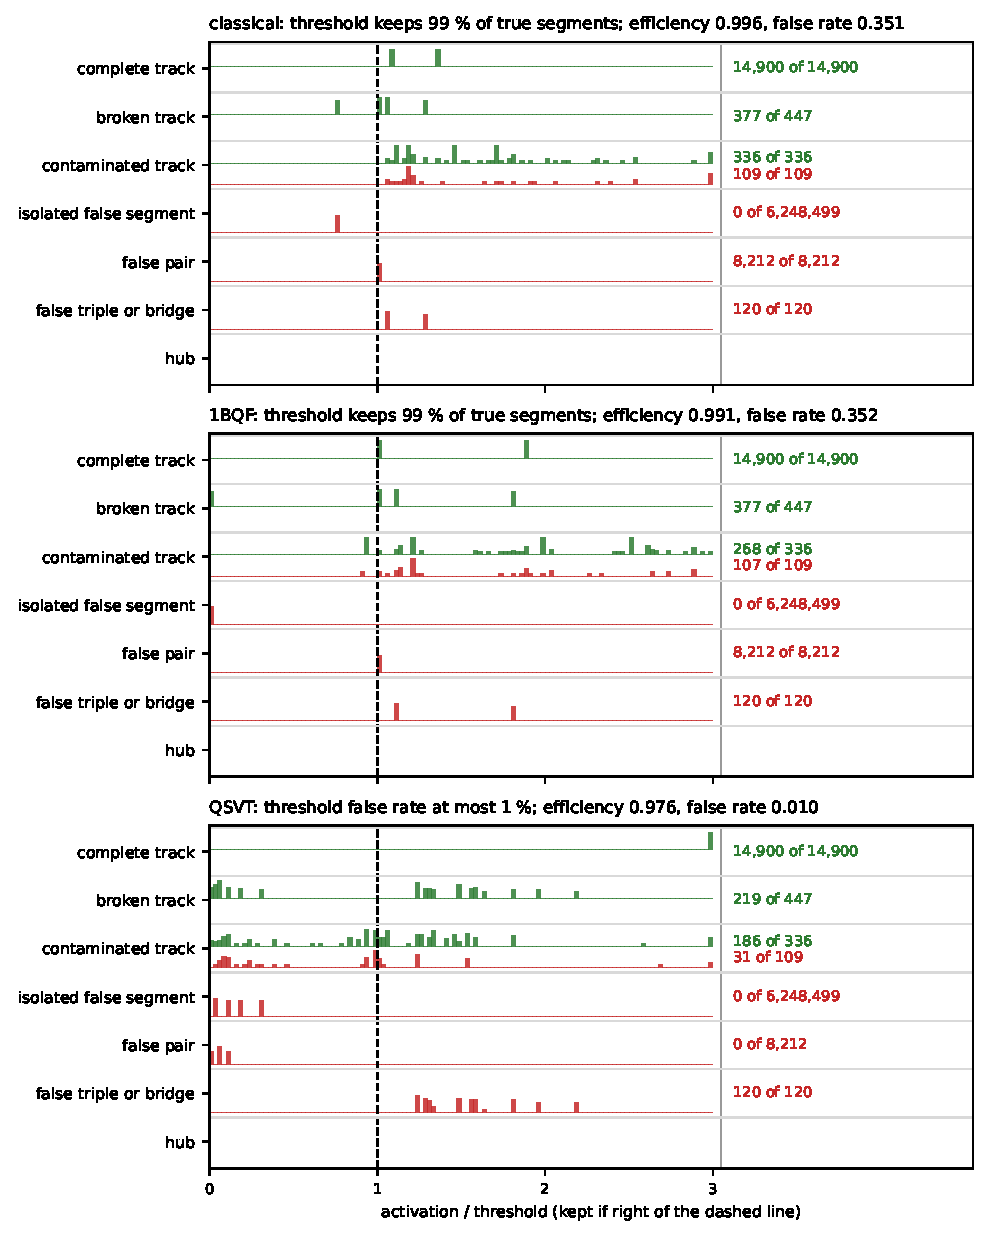
\includegraphics[width=0.92\textwidth]{fig3_error_atlas_T400_with_qsvt.pdf}
\caption{\gss{\textbf{Segment classes kept by each solver}, at 400 tracks pooled over $\NEvents$ events. The layout and the thresholds are those of figure~\ref{fig:atlas}.}}
\label{fig:atlas400}
\end{figure}

\begin{table}[H]
\centering\footnotesize
\caption{\gss{\textbf{Design scan.} Efficiency at a false rate of at most $1\%$ for each of the $\TeethNDesigns$ designs. A design is the set of passes, the degree and the half-width of each pass. The selection score is the mean over $T$ of the median efficiency on events 0 to 4. The held-out columns give the median efficiency on events 5 to 9 at 400, 700 and 1000 tracks. The rows are sorted by the selection score. $^\ast$: best design on events 0 to 4. $^\dagger$: design of the main text.}}
\label{tab:designs}
\begin{tabular}{lccrccc}\toprule
Passes & degree & half-width & selection, events 0--4 & \multicolumn{3}{c}{held out, events 5--9}\\
\cmidrule(lr){5-7}
 & & & & 400 & 700 & 1000\\\midrule
two bright$^\ast$ & 60 & 0.12 & 0.963 & 0.968 & 0.960 & 0.951\\
four & 24 & 0.30 & 0.963 & 0.973 & 0.941 & 0.933\\
four & 24 & 0.24 & 0.963 & 0.974 & 0.934 & 0.925\\
four & 60 & 0.12 & 0.962 & 0.958 & 0.960 & 0.937\\
two bright & 40 & 0.30 & 0.962 & 0.953 & 0.941 & 0.934\\
two bright & 60 & 0.30 & 0.962 & 0.953 & 0.941 & 0.934\\
four & 60 & 0.30 & 0.961 & 0.973 & 0.934 & 0.925\\
four & 40 & 0.24 & 0.960 & 0.974 & 0.935 & 0.925\\
four & 60 & 0.24 & 0.960 & 0.973 & 0.934 & 0.925\\
four & 24 & 0.18 & 0.960 & 0.965 & 0.934 & 0.925\\
four & 40 & 0.30 & 0.960 & 0.973 & 0.934 & 0.925\\
four$^\dagger$ & 40 & 0.18 & 0.960 & 0.970 & 0.935 & 0.928\\
four & 60 & 0.18 & 0.960 & 0.970 & 0.934 & 0.925\\
two bright & 40 & 0.18 & 0.960 & 0.970 & 0.934 & 0.925\\
two bright & 60 & 0.18 & 0.960 & 0.970 & 0.934 & 0.925\\
two bright & 24 & 0.18 & 0.959 & 0.970 & 0.934 & 0.928\\
two bright & 60 & 0.24 & 0.959 & 0.965 & 0.934 & 0.925\\
two bright & 40 & 0.24 & 0.959 & 0.965 & 0.934 & 0.925\\
two bright & 40 & 0.12 & 0.959 & 0.966 & 0.934 & 0.925\\
two bright & 24 & 0.30 & 0.958 & 0.958 & 0.937 & 0.934\\
two bright & 24 & 0.24 & 0.958 & 0.965 & 0.937 & 0.929\\
two bright & 24 & 0.12 & 0.958 & 0.970 & 0.934 & 0.925\\
four & 24 & 0.12 & 0.956 & 0.965 & 0.934 & 0.925\\
four & 40 & 0.12 & 0.953 & 0.965 & 0.934 & 0.934\\
two dark & 40 & 0.18 & 0.006 & 0.006 & 0.000 & 0.000\\
\bottomrule
\end{tabular}

\end{table}

\begin{table}[H]
\centering\footnotesize
\caption{\gss{\textbf{Post-selection probability against track multiplicity.} $P$ is the median over the $\NEvents$ events; rounds are the amplification rounds $\pi/(4\sqrt P)$. The values at 400 and 1000 tracks are those of table~\ref{tab:cost}.}}
\label{tab:P}
\begin{tabular}{rcccccc}\toprule
 & \multicolumn{2}{c}{One-bit filter} & \multicolumn{2}{c}{QSVT, phase sequence} & \multicolumn{2}{c}{QSVT, Chebyshev walk}\\
\cmidrule(lr){2-3}\cmidrule(lr){4-5}\cmidrule(lr){6-7}
$T$ & $P$ & rounds & $P$ & rounds & $P$ & rounds\\\midrule
10 & $3.37\times10^{-2}$ & 4 & $1.69\times10^{-2}$ & 6 & $4.42\times10^{-2}$ & 4\\
20 & $1.68\times10^{-2}$ & 6 & $8.33\times10^{-3}$ & 9 & $2.18\times10^{-2}$ & 5\\
50 & $6.64\times10^{-3}$ & 10 & $3.23\times10^{-3}$ & 14 & $8.46\times10^{-3}$ & 9\\
100 & $3.39\times10^{-3}$ & 13 & $1.63\times10^{-3}$ & 19 & $4.28\times10^{-3}$ & 12\\
200 & $1.78\times10^{-3}$ & 19 & $8.07\times10^{-4}$ & 28 & $2.14\times10^{-3}$ & 17\\
400 & $1.05\times10^{-3}$ & 24 & $4.15\times10^{-4}$ & 39 & $1.10\times10^{-3}$ & 24\\
700 & $8.49\times10^{-4}$ & 27 & $4.49\times10^{-4}$ & 37 & $1.44\times10^{-3}$ & 21\\
1000 & $8.60\times10^{-4}$ & 27 & $2.28\times10^{-4}$ & 52 & $7.25\times10^{-4}$ & 29\\
\bottomrule
\end{tabular}

\end{table}

\begin{table}[H]
\centering\footnotesize
\caption{\gss{\textbf{Configuration scan.} Efficiency at a false rate of at most $1\%$ of the three solvers, for four detector configurations. A configuration is the hit resolution, the kink per plane and the half-opening angle of the track cone. Every configuration loses $1\%$ of hits. Each entry is the median over $\ScanNEvents$ events; with two events, the median is the mean. The $5\,\mu$m rows are the configuration of the main text, read on $\ScanNEvents$ events instead of $\NEvents$.}}
\label{tab:scan}
\begin{tabular}{lcccc}\toprule
Configuration & $T$ & Classical & One-bit filter & Polynomial\\\midrule
$3\,\mu$m, $0.10$\,mrad, $0.2$\,rad & 200 & $\ScanClassThreeUmTwoHundred$ & $\ScanOneBitThreeUmTwoHundred$ & $\ScanQsvtThreeUmTwoHundred$\\
 & 400 & $\ScanClassThreeUmFourHundred$ & $\ScanOneBitThreeUmFourHundred$ & $\ScanQsvtThreeUmFourHundred$\\
 & 700 & $\ScanClassThreeUmSevenHundred$ & $\ScanOneBitThreeUmSevenHundred$ & $\ScanQsvtThreeUmSevenHundred$\\
 & 1000 & $\ScanClassThreeUmThousand$ & $\ScanOneBitThreeUmThousand$ & $\ScanQsvtThreeUmThousand$\\
\addlinespace
$5\,\mu$m, $0.15$\,mrad, $0.2$\,rad & 200 & $\ScanClassFiveUmTwoHundred$ & $\ScanOneBitFiveUmTwoHundred$ & $\ScanQsvtFiveUmTwoHundred$\\
 & 400 & $\ScanClassFiveUmFourHundred$ & $\ScanOneBitFiveUmFourHundred$ & $\ScanQsvtFiveUmFourHundred$\\
 & 700 & $\ScanClassFiveUmSevenHundred$ & $\ScanOneBitFiveUmSevenHundred$ & $\ScanQsvtFiveUmSevenHundred$\\
 & 1000 & $\ScanClassFiveUmThousand$ & $\ScanOneBitFiveUmThousand$ & $\ScanQsvtFiveUmThousand$\\
\addlinespace
$10\,\mu$m, $0.30$\,mrad, $0.2$\,rad & 200 & $\ScanClassTenUmTwoHundred$ & $\ScanOneBitTenUmTwoHundred$ & $\ScanQsvtTenUmTwoHundred$\\
 & 400 & $\ScanClassTenUmFourHundred$ & $\ScanOneBitTenUmFourHundred$ & $\ScanQsvtTenUmFourHundred$\\
 & 700 & $\ScanClassTenUmSevenHundred$ & $\ScanOneBitTenUmSevenHundred$ & $\ScanQsvtTenUmSevenHundred$\\
 & 1000 & $\ScanClassTenUmThousand$ & $\ScanOneBitTenUmThousand$ & $\ScanQsvtTenUmThousand$\\
\addlinespace
$15\,\mu$m, $0.45$\,mrad, $0.4$\,rad & 200 & $\ScanClassFifteenUmTwoHundred$ & $\ScanOneBitFifteenUmTwoHundred$ & $\ScanQsvtFifteenUmTwoHundred$\\
 & 400 & $\ScanClassFifteenUmFourHundred$ & $\ScanOneBitFifteenUmFourHundred$ & $\ScanQsvtFifteenUmFourHundred$\\
 & 700 & $\ScanClassFifteenUmSevenHundred$ & $\ScanOneBitFifteenUmSevenHundred$ & $\ScanQsvtFifteenUmSevenHundred$\\
 & 1000 & $\ScanClassFifteenUmThousand$ & $\ScanOneBitFifteenUmThousand$ & $\ScanQsvtFifteenUmThousand$\\
\bottomrule
\end{tabular}
\end{table}

\end{document}
